\documentclass[a4paper,14pt]{extarticle}
\usepackage{../../../template/gostreport}
\providecommand{\tightlist}{\setlength{\itemsep}{0pt}\setlength{\parskip}{0pt}}
\usepackage{adjustbox}
\usepackage{hyperref}
\hypersetup{hidelinks}
\begin{document}
\makegosttitle
  {2}
  {2D-преобразования}
  {студент группы R3243 Осипов А.\,П.\\[4pt]
   студент группы R3243 Глазков В.\\[4pt]
   студент группы R3243 Прохоревич И.}
  {Догадин Е.\,В.}
\tableofcontents
\newpage
\unnumsection{Введение}
Цель работы --- изучить матрицы $2\times 2$ как линейные отображения плоскости: построить матрицы с заданными геометрическими свойствами, визуализировать их действие на многоугольник и проанализировать ядро, образ, собственные числа и определители.

\hypertarget{ux438ux441ux445ux43eux434ux43dux44bux435-ux434ux430ux43dux43dux44bux435}{%
\section{Исходные
данные}\label{ux438ux441ux445ux43eux434ux43dux44bux435-ux434ux430ux43dux43dux44bux435}}

Выбираем вместе один раз, дальше не меняем. Те же значения --- в
\texttt{code/common.py}.

\begin{itemize}
\tightlist
\item
  a = 3
\item
  b = -2
\item
  c = 4
\item
  d = 14
\item
  как выбраны: почитав задания решено выбирать максимально информативные
  числа, в то же время случайные, a и b были выбраны небольшими по
  модулю чтобы коэфф угла наклона был небольшим, так удобнее наблюдать
  за наклоном. c и d повороты, а также площадь круга в п.9 и некруга в
  п.10 соответственно (поэтому в дальнейшем выбраны положительные),
  выбрал 4 и 14 чтобы задания получились содержательными и не попадали в
  исключительно удобные случаи 90deg 180deg 360deg etc. важно упомянуть
  числа выбраны с учётом ограничений методички и так, чтобы ни один
  пункт не вырождался.
\item
  многоугольник (вершины): девятиугольник «рыба» без осей симметрии ---
  A(−4, 0), B(−2, 1), C(0, 1), D(1, 0), E(3, 3), F(3, −2), G(1, −1),
  H(−1, −2), I(−3, −1)
\end{itemize}

\hypertarget{ux432ux44bux43fux43eux43bux43dux435ux43dux438ux435-ux440ux430ux431ux43eux442ux44b}{%
\section{Выполнение
работы}\label{ux432ux44bux43fux43eux43bux43dux435ux43dux438ux435-ux440ux430ux431ux43eux442ux44b}}

\hypertarget{ux43fux443ux43dux43aux442-1.-ux43eux442ux440ux430ux436ux435ux43dux438ux435-ux43eux442ux43dux43eux441ux438ux442ux435ux43bux44cux43dux43e-y-ax}{%
\subsection{Пункт 1. Отражение относительно y =
ax}\label{ux43fux443ux43dux43aux442-1.-ux43eux442ux440ux430ux436ux435ux43dux438ux435-ux43eux442ux43dux43eux441ux438ux442ux435ux43bux44cux43dux43e-y-ax}}

\textbf{Общий класс.} Чтобы найти матрицу, достаточно знать, куда она
переводит два неколлинеарных вектора. Для отражения такие векторы
известны заранее:

\begin{itemize}
\tightlist
\item
  \(u = (1, a)^T\) лежит на прямой \(y = ax\) --- зеркало его не меняет:
  \(Mu = u\);
\item
  \(w = (-a, 1)^T\) перпендикулярен прямой (\(u \cdot w = -a + a = 0\))
  --- зеркало его переворачивает: \(Mw = -w = (a, -1)^T\).
\end{itemize}

Составим из векторов матрицы по столбцам: \(P = (u \;\; w)\),
\(Q = (Mu \;\; Mw) = (u \;\; -w)\). Так как умножение на \(M\) действует
на каждый столбец отдельно, \(MP = Q\), откуда \(M = QP^{-1}\) (умножаем
на \(P^{-1}\) справа, порядок важен --- матрицы не коммутируют).

\begin{center}\adjustbox{max width=\linewidth}{$\displaystyle P = \begin{pmatrix} 1 & -a \\ a & 1 \end{pmatrix}, \quad
\det P = 1 + a^2,$}\end{center}

\begin{center}\adjustbox{max width=\linewidth}{$\displaystyle P^{-1} = \frac{1}{1 + a^2}\begin{pmatrix} 1 & a \\ -a & 1 \end{pmatrix}, \quad
Q = \begin{pmatrix} 1 & a \\ a & -1 \end{pmatrix}$}\end{center}

\begin{center}\adjustbox{max width=\linewidth}{$\displaystyle M = QP^{-1} = \frac{1}{1 + a^2}\begin{pmatrix} 1 - a^2 & 2a \\ 2a & a^2 - 1 \end{pmatrix}$}\end{center}

\textbf{Выбранная матрица.} При \(a = 3\): \(\det P = 10\),

\begin{center}\adjustbox{max width=\linewidth}{$\displaystyle P^{-1} = \frac{1}{10}\begin{pmatrix} 1 & 3 \\ -3 & 1 \end{pmatrix},$}\end{center}

\begin{center}\adjustbox{max width=\linewidth}{$\displaystyle M_1 = \begin{pmatrix} 1 & 3 \\ 3 & -1 \end{pmatrix} \cdot \frac{1}{10}\begin{pmatrix} 1 & 3 \\ -3 & 1 \end{pmatrix}
= \frac{1}{10}\begin{pmatrix} -8 & 6 \\ 6 & 8 \end{pmatrix}
= \begin{pmatrix} -0.8 & 0.6 \\ 0.6 & 0.8 \end{pmatrix}$}\end{center}

Проверка: \(M_1 u = (-0.8 + 1.8,\; 0.6 + 2.4) = (1, 3) = u\),
\(M_1 w = (2.4 + 0.6,\; -1.8 + 0.8) = (3, -1) = -w\).

\textbf{Визуализация.} Результат показан на рисунке~\ref{fig:p01}.

\begin{figure}[H]
\centering
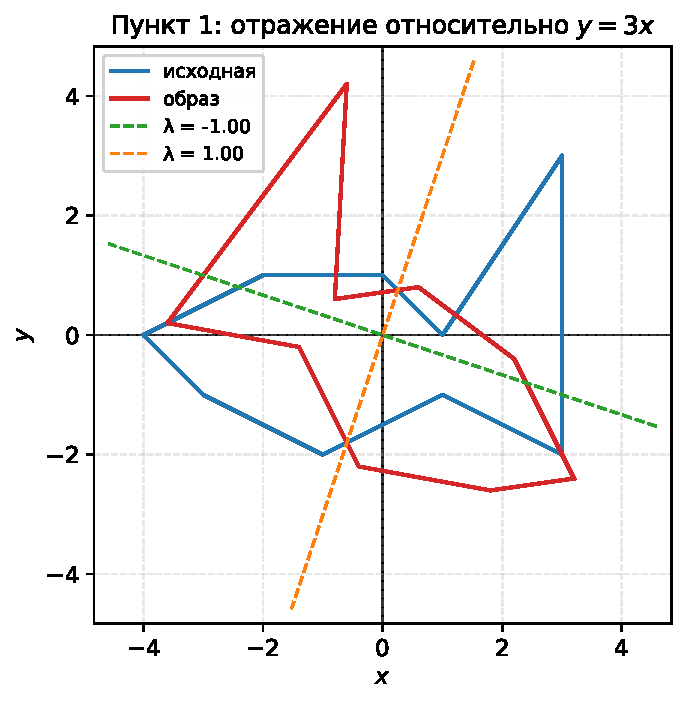
\includegraphics[width=0.55\textwidth]{../figures/p01.pdf}
\caption{Отражение многоугольника относительно прямой y = 3x; пунктиром
--- собственные направления}
\label{fig:p01}
\end{figure}

\textbf{Анализ (задание 2).}

\emph{Собственные числа и векторы.} Ищем из \(Mv = \lambda v\), то есть
\((M - \lambda I)v = 0\); ненулевое решение есть, только если
\(\det(M - \lambda I) = 0\):

\begin{center}\adjustbox{max width=\linewidth}{$\displaystyle \det\begin{pmatrix} -0.8 - \lambda & 0.6 \\ 0.6 & 0.8 - \lambda \end{pmatrix}
= \lambda^2 - 0.64 - 0.36 = \lambda^2 - 1 = 0 \;\Rightarrow\; \lambda_{1,2} = \pm 1.$}\end{center}

Подставляя каждое \(\lambda\) в \((M - \lambda I)v = 0\), получаем
\(\lambda_1 = 1\): \(v_1 = (1, 3)^T\) --- вдоль прямой \(y = 3x\);
\(\lambda_2 = -1\): \(v_2 = (-3, 1)^T\) --- перпендикулярно ей. Это
ровно векторы \(u\) и \(w\), из которых строилась матрица.

\emph{Определитель.} \(\det M_1 = (-0.8)(0.8) - 0.6 \cdot 0.6 = -1\).
Модуль 1 --- площадь фигуры не меняется. Знак минус --- отражение меняет
ориентацию плоскости: образы базисных векторов меняются сторонами (образ
первого оказывается «левее» образа второго), плоскость как бы
переворачивается.

\emph{Ядро и образ.} \(\det M_1 \ne 0\), значит ранг равен 2 (числу
столбцов), и размерность ядра \(2 - 2 = 0\): \(\ker M_1 = \{0\}\) ---
никакой ненулевой вектор не переходит в ноль. Образ --- все линейные
комбинации столбцов, его размерность равна рангу:
\(\operatorname{Im} M_1 = \mathbb{R}^2\).

матрица симметрична так как она при транспонировании она совпадает с
дефолтной (элементы b \& c равны) инволютивна так как она она отражает
без изменения длины векторов и если дважды отразить то вектор останется
прежним ортогональна так при умножении ее на транспонированную
получается единичная матрица, то есть длины и углы сохраняются

\textbf{Вывод.}

собственные числа = +-1 показывают во сколько раз меняется вектор
лежащий на собственном векторе, так как у нас определитель -1, Площадь
не меняется, потому что \textbar det\textbar{} = 1, но вектор лежащий на
собственном векторе с собственным числом 1 не меняет направление и не
меняет длину, а вектор лежащий на векторе с сч -1 меняет направление но
не меняет длину. определитель -1 так как базисные векторы меняются
сторонами, то есть базисный вектор 1 становится левее чем базисный
вектор 2, пространство переворачивается, это и есть знак -. у св и
прямой-зеркала есть общее: как раз св с сч 1 лежит на этом зеркале, а
иной св перпендикулярен ему.

\hypertarget{ux43fux443ux43dux43aux442-2.-ux43eux440ux442ux43eux433ux43eux43dux430ux43bux44cux43dux430ux44f-ux43fux440ux43eux435ux43aux446ux438ux44f-ux43dux430-y-bx}{%
\subsection{Пункт 2. Ортогональная проекция на y =
bx}\label{ux43fux443ux43dux43aux442-2.-ux43eux440ux442ux43eux433ux43eux43dux430ux43bux44cux43dux430ux44f-ux43fux440ux43eux435ux43aux446ux438ux44f-ux43dux430-y-bx}}

\textbf{Общий класс.} Тот же приём, что в пункте 1. Берём
\(u = (1, b)^T\) на прямой \(y = bx\) и \(w = (-b, 1)^T\),
перпендикулярный ей. Ортогональная проекция оставляет \(u\) на месте, а
\(w\) переводит в ноль: перпендикуляр из конца \(w\) падает в начало
координат. Тогда \(Mu = u\), \(Mw = 0\), и из \(MP = Q\):

\begin{center}\adjustbox{max width=\linewidth}{$\displaystyle P = \begin{pmatrix} 1 & -b \\ b & 1 \end{pmatrix}, \quad
Q = \begin{pmatrix} 1 & 0 \\ b & 0 \end{pmatrix},$}\end{center}

\begin{center}\adjustbox{max width=\linewidth}{$\displaystyle M = QP^{-1} = \frac{1}{1 + b^2}\begin{pmatrix} 1 & b \\ b & b^2 \end{pmatrix}$}\end{center}

\textbf{Выбранная матрица.} При \(b = -2\): \(\det P = 5\),

\begin{center}\adjustbox{max width=\linewidth}{$\displaystyle P^{-1} = \frac{1}{5}\begin{pmatrix} 1 & -2 \\ 2 & 1 \end{pmatrix},$}\end{center}

\begin{center}\adjustbox{max width=\linewidth}{$\displaystyle M_2 = \begin{pmatrix} 1 & 0 \\ -2 & 0 \end{pmatrix} \cdot \frac{1}{5}\begin{pmatrix} 1 & -2 \\ 2 & 1 \end{pmatrix}
= \frac{1}{5}\begin{pmatrix} 1 & -2 \\ -2 & 4 \end{pmatrix}
= \begin{pmatrix} 0.2 & -0.4 \\ -0.4 & 0.8 \end{pmatrix}$}\end{center}

Проверка: \(M_2 u = (0.2 + 0.8,\; -0.4 - 1.6) = (1, -2) = u\),
\(M_2 w = (0.4 - 0.4,\; -0.8 + 0.8) = (0, 0)\).

\textbf{Визуализация.} Результат показан на рисунке~\ref{fig:p02}: весь
многоугольник схлопывается в отрезок на прямой \(y = -2x\).

\begin{figure}[H]
\centering
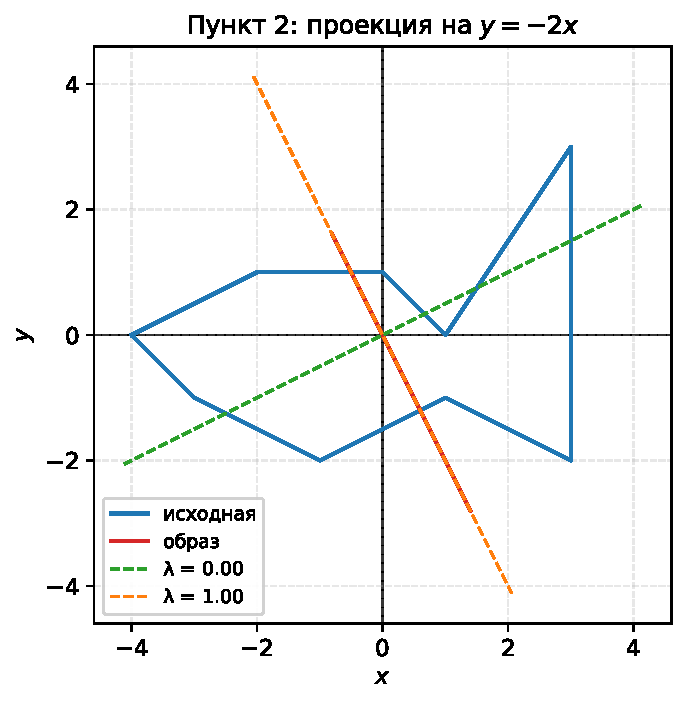
\includegraphics[width=0.55\textwidth]{../figures/p02.pdf}
\caption{Ортогональная проекция многоугольника на прямую y = −2x;
пунктиром --- собственные направления}
\label{fig:p02}
\end{figure}

\textbf{Анализ (задание 2).}

\emph{Собственные числа и векторы.}

\begin{center}\adjustbox{max width=\linewidth}{$\displaystyle \det(M_2 - \lambda I) = (0.2 - \lambda)(0.8 - \lambda) - 0.16 = \lambda^2 - \lambda = \lambda(\lambda - 1) = 0
\;\Rightarrow\; \lambda_1 = 1,\; \lambda_2 = 0.$}\end{center}

\(\lambda_1 = 1\): \(v_1 = (1, -2)^T\) --- векторы на прямой проекции не
меняются. \(\lambda_2 = 0\): \(v_2 = (2, 1)^T\) --- векторы,
перпендикулярные прямой, обнуляются.

\emph{Определитель.} \(\det M_2 = 0.2 \cdot 0.8 - (-0.4)^2 = 0\).
Матрица вырождена: она схлопывает всю плоскость в прямую, а площадь
любой фигуры на прямой равна нулю.

\emph{Ядро и образ.} Ранг --- максимальное число линейно независимых
столбцов; оба столбца \(M_2\) пропорциональны \((1, -2)^T\), поэтому
\(\operatorname{rank} M_2 = 1 < 2\), и матрица обнуляет некоторые
ненулевые векторы. Из \(M_2 (x, y)^T = 0\): \(0.2x - 0.4y = 0\), то есть
\(x = 2y\):

\begin{center}\adjustbox{max width=\linewidth}{$\displaystyle \ker M_2 = \{ t\,(2, 1)^T \} \text{ — прямая } y = -\tfrac{1}{b}x = \tfrac{x}{2}, \qquad
\operatorname{Im} M_2 = \{ t\,(1, -2)^T \} \text{ — прямая } y = bx = -2x.$}\end{center}

Размерности: \(\dim\ker + \dim\operatorname{Im} = 1 + 1 = 2\).

\emph{Свойства.} Матрица \textbf{симметрична}: \(M_2^T = M_2\).
\textbf{Не инволютивна}: повторная проекция ничего не меняет, вектор
остаётся спроецированным, поэтому \(M_2^2 = M_2 \ne I\). \textbf{Не
ортогональна}: \(M_2^T M_2 = M_2 \ne I\), длины и углы не сохраняются.

\textbf{Вывод.} Определитель равен нулю: проекция схлопывает плоскость в
прямую, и у образа фигуры нет площади. Собственные числа 0 и 1
соответствуют двум особым направлениям: векторы, перпендикулярные
прямой, обнуляются, а векторы на самой прямой не меняются. Проекция идёт
как раз на прямую собственного вектора с \(\lambda = 1\), а ядро --- это
прямая собственного вектора с \(\lambda = 0\).

\hypertarget{ux43fux443ux43dux43aux442-3.-ux43fux43eux432ux43eux440ux43eux442-ux43dux430-10c-ux43fux440ux43eux442ux438ux432-ux447ux430ux441ux43eux432ux43eux439}{%
\subsection{Пункт 3. Поворот на 10c° против
часовой}\label{ux43fux443ux43dux43aux442-3.-ux43fux43eux432ux43eux440ux43eux442-ux43dux430-10c-ux43fux440ux43eux442ux438ux432-ux447ux430ux441ux43eux432ux43eux439}}

\textbf{Общий класс.} При повороте на угол \(\varphi\) против часовой
базисный вектор \((1, 0)^T\) переходит в
\((\cos\varphi, \sin\varphi)^T\), а \((0, 1)^T\) --- в
\((-\sin\varphi, \cos\varphi)^T\). Образы базисных векторов --- это
столбцы матрицы, поэтому

\begin{center}\adjustbox{max width=\linewidth}{$\displaystyle R(\varphi) = \begin{pmatrix} \cos\varphi & -\sin\varphi \\ \sin\varphi & \cos\varphi \end{pmatrix}.$}\end{center}

Матрица поворота на заданный угол единственна: угол полностью
определяет, куда идут оба базисных вектора.

\textbf{Выбранная матрица.} При \(c = 4\) угол
\(\varphi = 10c = 40^\circ\):

\begin{center}\adjustbox{max width=\linewidth}{$\displaystyle M_3 = R(40^\circ) = \begin{pmatrix} \cos 40^\circ & -\sin 40^\circ \\ \sin 40^\circ & \cos 40^\circ \end{pmatrix}
\approx \begin{pmatrix} 0.766 & -0.643 \\ 0.643 & 0.766 \end{pmatrix}$}\end{center}

\textbf{Визуализация.} Результат показан на рисунке~\ref{fig:p03}. Собственных
прямых на рисунке нет --- вещественных собственных векторов у поворота
нет.

\begin{figure}[H]
\centering
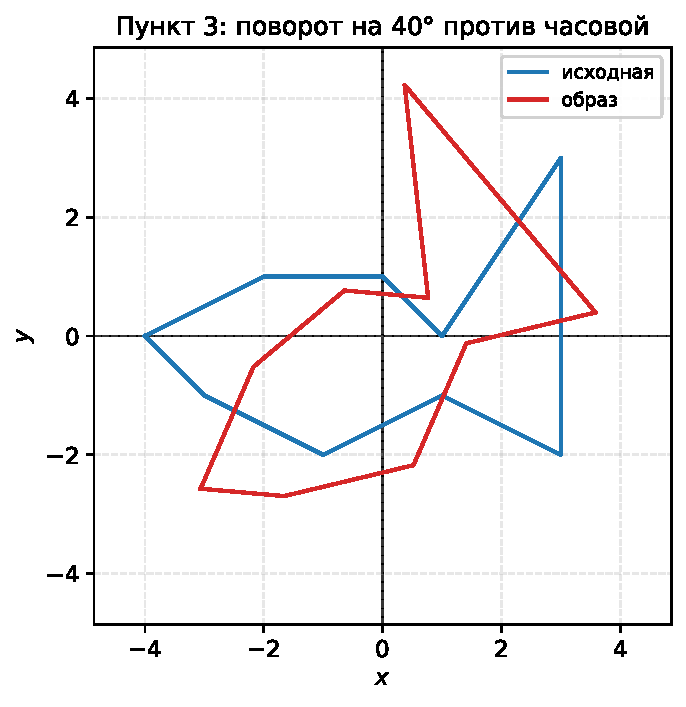
\includegraphics[width=0.55\textwidth]{../figures/p03.pdf}
\caption{Поворот многоугольника на 40° против часовой стрелки}
\label{fig:p03}
\end{figure}

\textbf{Анализ (задание 2).}

\emph{Собственные числа и векторы.}

\begin{center}\adjustbox{max width=\linewidth}{$\displaystyle \det(R - \lambda I) = (\cos\varphi - \lambda)^2 + \sin^2\varphi = 0
\;\Rightarrow\; \lambda_{1,2} = \cos\varphi \pm i\sin\varphi = e^{\pm i\varphi}.$}\end{center}

При \(\varphi = 40^\circ\): \(\lambda_{1,2} \approx 0.766 \pm 0.643i\).
Вещественных собственных чисел нет, поэтому нет и вещественных
собственных векторов: поворот на \(40^\circ\) меняет направление любого
ненулевого вектора, ни одна прямая через начало координат не остаётся на
месте. Собственные векторы есть только комплексные, на вещественной
плоскости их нарисовать нельзя.

\emph{Определитель.}
\(\det M_3 = \cos^2 40^\circ + \sin^2 40^\circ = 1\): поворот не
растягивает и не сжимает плоскость (площадь сохраняется) и не меняет
ориентацию.

\emph{Свойства.} \textbf{Не симметрична}
(\(-\sin 40^\circ \ne \sin 40^\circ\)). \textbf{Не инволютивна}:
\(M_3^2 = R(80^\circ) \ne I\). \textbf{Ортогональна}:
\(M_3^T M_3 = R(-40^\circ) R(40^\circ) = I\) --- длины и углы
сохраняются.

\textbf{Вывод.} Поворот --- ортогональное преобразование с определителем
\(+1\): оно сохраняет и площади, и ориентацию. Вещественных собственных
векторов нет, потому что при повороте на угол, не кратный \(180^\circ\),
каждый вектор меняет направление; собственные числа \(e^{\pm i\varphi}\)
комплексно-сопряжённые и по модулю равны 1.

\hypertarget{ux43fux443ux43dux43aux442-4.-ux446ux435ux43dux442ux440ux430ux43bux44cux43dux430ux44f-ux441ux438ux43cux43cux435ux442ux440ux438ux44f}{%
\subsection{Пункт 4. Центральная
симметрия}\label{ux43fux443ux43dux43aux442-4.-ux446ux435ux43dux442ux440ux430ux43bux44cux43dux430ux44f-ux441ux438ux43cux43cux435ux442ux440ux438ux44f}}

\textbf{Общий класс.} Центральная симметрия переводит каждую точку в
точку по другую сторону от начала координат на том же расстоянии:
\(v \mapsto -v\), то есть все координаты меняют знак. Значит,
\((1, 0)^T \mapsto (-1, 0)^T\), \((0, 1)^T \mapsto (0, -1)^T\), и
матрица единственна:

\begin{center}\adjustbox{max width=\linewidth}{$\displaystyle M_4 = -I = \begin{pmatrix} -1 & 0 \\ 0 & -1 \end{pmatrix}.$}\end{center}

Это то же самое, что поворот на \(180^\circ\): \(R(180^\circ) = -I\).

\textbf{Выбранная матрица.} \(M_4 = -I\) (других вариантов нет).

\textbf{Визуализация.} Результат показан на рисунке~\ref{fig:p04}.

\begin{figure}[H]
\centering
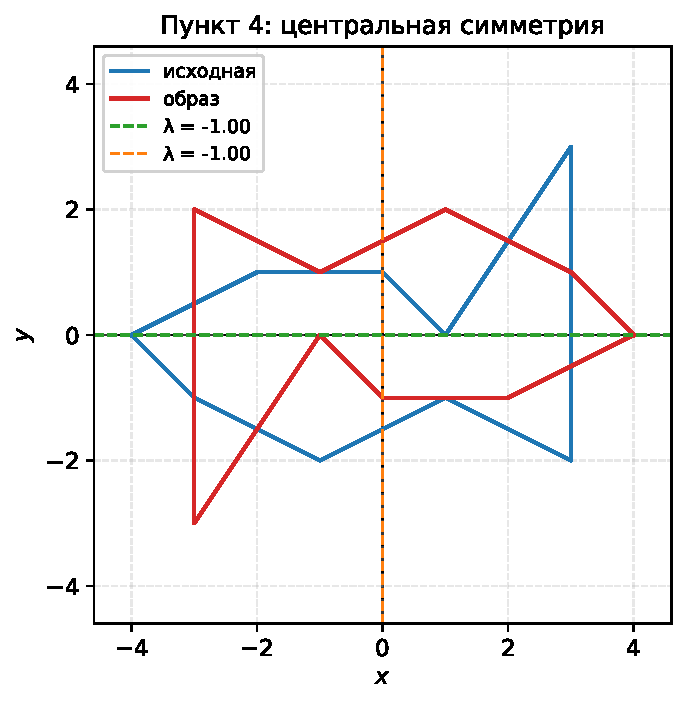
\includegraphics[width=0.55\textwidth]{../figures/p04.pdf}
\caption{Центральная симметрия многоугольника относительно начала
координат}
\label{fig:p04}
\end{figure}

\textbf{Анализ (задание 2).}

\emph{Собственные числа и векторы.}
\(\det(M_4 - \lambda I) = (-1 - \lambda)^2 = 0\), \(\lambda_{1,2} = -1\)
(кратность 2). Любой ненулевой вектор собственный: \(M_4 v = -v\) ---
вектор остаётся на своей прямой, только разворачивается в
противоположную сторону. Собственное пространство --- вся плоскость,
геометрическая кратность равна алгебраической: 2.

\emph{Определитель.} \(\det M_4 = (-1)(-1) - 0 = 1\). Площадь
сохраняется, ориентация тоже: несмотря на то, что каждый вектор
«переворачивается», это поворот на \(180^\circ\), а не отражение.

\emph{Свойства.} \textbf{Симметрична} (\(M_4^T = M_4\)),
\textbf{инволютивна} (\(M_4^2 = I\) --- дважды отразить относительно
центра значит вернуться), \textbf{ортогональна} (\(M_4^T M_4 = I\)).

\textbf{Вывод.} Центральная симметрия на плоскости --- это поворот на
\(180^\circ\), поэтому её определитель \(+1\), а не \(-1\): две смены
знака (по каждой оси) дают сохранение ориентации. Все векторы
собственные с \(\lambda = -1\), потому что каждый остаётся на своей
прямой.

\hypertarget{ux43fux443ux43dux43aux442-5.-ux43eux442ux440ux430ux436ux435ux43dux438ux435-ux43eux442ux43dux43eux441ux438ux442ux435ux43bux44cux43dux43e-y-ax-ux437ux430ux442ux435ux43c-ux43fux43eux432ux43eux440ux43eux442-ux43dux430-10d-ux43fux43e-ux447ux430ux441ux43eux432ux43eux439}{%
\subsection{Пункт 5. Отражение относительно y = ax, затем поворот на
10d° по
часовой}\label{ux43fux443ux43dux43aux442-5.-ux43eux442ux440ux430ux436ux435ux43dux438ux435-ux43eux442ux43dux43eux441ux438ux442ux435ux43bux44cux43dux43e-y-ax-ux437ux430ux442ux435ux43c-ux43fux43eux432ux43eux440ux43eux442-ux43dux430-10d-ux43fux43e-ux447ux430ux441ux43eux432ux43eux439}}

\textbf{Общий класс.} Поворот по часовой на угол \(\alpha\) --- это
поворот против часовой на \(-\alpha\): \(R(-\alpha)\). Отображение
применяется к вектору справа налево: сначала отражение \(M_1\), потом
поворот, \(M_5 v = R(-\alpha)(M_1 v)\), поэтому

\begin{center}\adjustbox{max width=\linewidth}{$\displaystyle M_5 = R(-\alpha)\, M_1.$}\end{center}

\textbf{Выбранная матрица.} При \(d = 14\):
\(\alpha = 10d = 140^\circ\),

\begin{center}\adjustbox{max width=\linewidth}{$\displaystyle M_5 = R(-140^\circ)\, M_1 \approx
\begin{pmatrix} -0.766 & 0.643 \\ -0.643 & -0.766 \end{pmatrix}
\begin{pmatrix} -0.8 & 0.6 \\ 0.6 & 0.8 \end{pmatrix}
\approx \begin{pmatrix} 0.999 & 0.055 \\ 0.055 & -0.999 \end{pmatrix}$}\end{center}

\textbf{Визуализация.} Результат показан на рисунке~\ref{fig:p05}.

\begin{figure}[H]
\centering
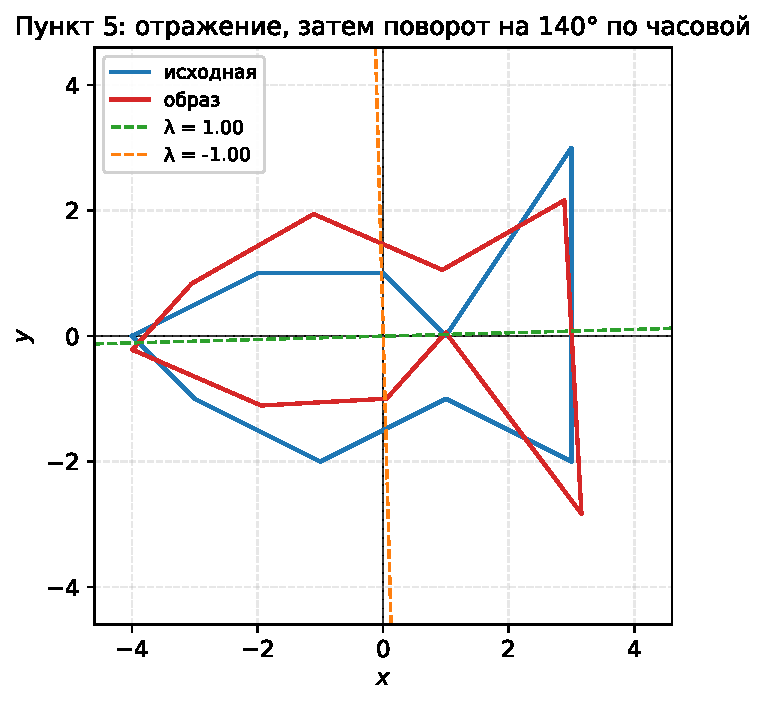
\includegraphics[width=0.55\textwidth]{../figures/p05.pdf}
\caption{Отражение относительно y = 3x, затем поворот на 140° по часовой
стрелке}
\label{fig:p05}
\end{figure}

\textbf{Анализ (задание 2).}

\emph{Определитель.} Определитель произведения равен произведению
определителей:
\(\det M_5 = \det R(-140^\circ) \cdot \det M_1 = 1 \cdot (-1) = -1\).
Ориентация меняется, площадь сохраняется.

\textbf{Вывод.} Отражение, за которым следует поворот, имеет
определитель \(-1\) и остаётся ортогональным преобразованием --- значит,
это снова отражение, только относительно другой прямой. Это видно и по
собственным числам, которые вычисляет программа: \(\lambda = \pm 1\).

\hypertarget{ux43fux443ux43dux43aux442-6.-y-0-y-ax-x-0-y-bx}{%
\subsection{Пункт 6. y = 0 → y = ax, x = 0 → y =
bx}\label{ux43fux443ux43dux43aux442-6.-y-0-y-ax-x-0-y-bx}}

\textbf{Общий класс.}

Пусть линейное отображение задаётся матрицей
\(M = \begin{bmatrix} p & q \\ r & s \end{bmatrix}\). Прямая \(y = 0\)
состоит из векторов вида \(\begin{bmatrix} t \\ 0 \end{bmatrix}\). Их
образ:
\begin{center}\adjustbox{max width=\linewidth}{$\displaystyle M \begin{bmatrix} t \\ 0 \end{bmatrix} = t \begin{bmatrix} p \\ r \end{bmatrix}$}\end{center}
Чтобы образ лежал на прямой \(y = ax\), первый столбец матрицы должен
быть коллинеарен вектору \(\begin{bmatrix} 1 \\ a \end{bmatrix}\), то
есть \(r = ap\).

Аналогично, прямая \(x = 0\) состоит из векторов
\(\begin{bmatrix} 0 \\ t \end{bmatrix}\). Их образ:
\begin{center}\adjustbox{max width=\linewidth}{$\displaystyle M \begin{bmatrix} 0 \\ t \end{bmatrix} = t \begin{bmatrix} q \\ s \end{bmatrix}$}\end{center}
Чтобы образ лежал на прямой \(y = bx\), второй столбец должен быть
коллинеарен вектору \(\begin{bmatrix} 1 \\ b \end{bmatrix}\), то есть
\(s = bq\).

Чтобы прямые переходили именно в прямые (а не в ноль), требуется
\(p \neq 0\) и \(q \neq 0\). Общий вид матрицы:
\begin{center}\adjustbox{max width=\linewidth}{$\displaystyle M = \begin{bmatrix} p & q \\ ap & bq \end{bmatrix}, \quad p,q \neq 0$}\end{center}
Определитель такой матрицы: \(\det M = p(bq) - q(ap) = pq(b - a)\). При
заданных \(a = 3\), \(b = -2\):
\begin{center}\adjustbox{max width=\linewidth}{$\displaystyle M = \begin{bmatrix} p & q \\ 3p & -2q \end{bmatrix}, \quad \det M = -5pq$}\end{center}

\textbf{Выбранная матрица.}

Возьмём простейший случай \(p = 1, q = 1\):
\begin{center}\adjustbox{max width=\linewidth}{$\displaystyle A = \begin{bmatrix} 1 & 1 \\ 3 & -2 \end{bmatrix}$}\end{center} Определитель:
\(\det A = 1 \cdot (-2) - 1 \cdot 3 = -5 \neq 0\).

\textbf{Визуализация.}

\begin{figure}[H]
\centering
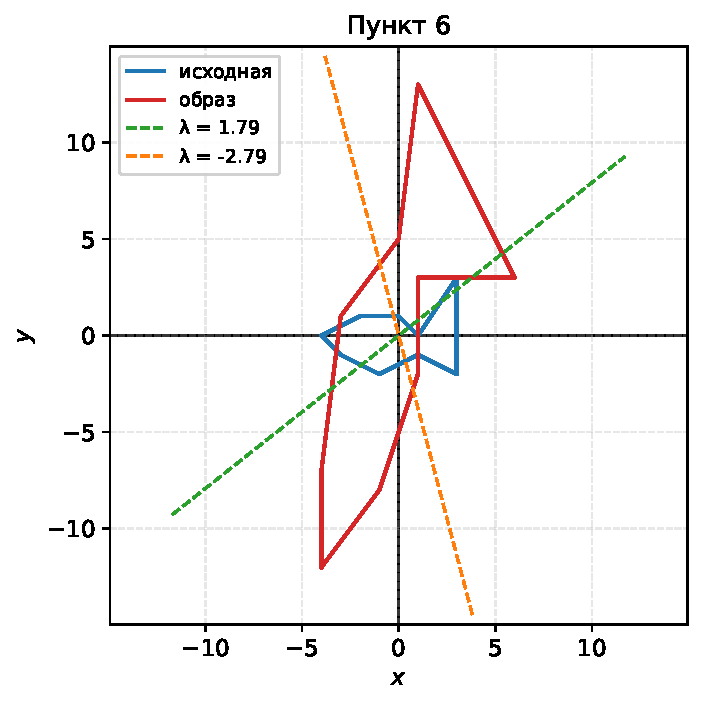
\includegraphics[width=0.55\textwidth]{../figures/p06.pdf}
\caption{Отображение пункта 6: исходный и отображённый многоугольник}
\label{fig:p06}
\end{figure}

\textbf{Анализ (задание 2).}

\emph{Определитель, ядро и образ:} \(\det A = -5\). Так как определитель
не равен нулю, отображение невырождено. Ядро:
\(\ker A = \{ \mathbf{0} \}\). Образ:
\(\operatorname{Im} A = \mathbb{R}^2\).

\emph{Собственные числа:} Характеристический многочлен:
\begin{center}\adjustbox{max width=\linewidth}{$\displaystyle \det(A - \lambda I) = \begin{vmatrix} 1 - \lambda & 1 \\ 3 & -2 - \lambda \end{vmatrix} = (1 - \lambda)(-2 - \lambda) - 3 = \lambda^2 + \lambda - 5$}\end{center}
Корни уравнения \(\lambda^2 + \lambda - 5 = 0\):
\begin{center}\adjustbox{max width=\linewidth}{$\displaystyle \lambda_{1,2} = \frac{-1 \pm \sqrt{1 + 20}}{2} = \frac{-1 \pm \sqrt{21}}{2}$}\end{center}

\emph{Собственные векторы:} Для собственного числа \(\lambda\) решаем
систему \((A - \lambda I)v = 0\). Из первого уравнения
\((1 - \lambda)x + y = 0\) получаем \(y = (\lambda - 1)x\). Собственный
вектор \(v = \begin{bmatrix} 1 \\ \lambda - 1 \end{bmatrix}\). Для
\(\lambda_1 = \frac{-1 + \sqrt{21}}{2}\):
\begin{center}\adjustbox{max width=\linewidth}{$\displaystyle v_1 = \begin{bmatrix} 1 \\ \frac{\sqrt{21} - 3}{2} \end{bmatrix}$}\end{center}
Для \(\lambda_2 = \frac{-1 - \sqrt{21}}{2}\):
\begin{center}\adjustbox{max width=\linewidth}{$\displaystyle v_2 = \begin{bmatrix} 1 \\ \frac{-\sqrt{21} - 3}{2} \end{bmatrix}$}\end{center}

\textbf{Вывод.}

Матрица \(A\) удовлетворяет условию, так как её столбцы
\(\begin{bmatrix} 1 \\ 3 \end{bmatrix}\) и
\(\begin{bmatrix} 1 \\ -2 \end{bmatrix}\) лежат на прямых \(y = 3x\) и
\(y = -2x\) соответственно, что геометрически означает перевод осей
координат в заданные прямые. Определитель \(\det A = -5 < 0\), что
означает изменение ориентации плоскости (отражение составляющей
преобразования). Модуль определителя \(|\det A| = 5\) показывает, что
площадь любого многоугольника при данном отображении увеличивается в 5
раз. Наличие двух вещественных собственных векторов подтверждает, что
преобразование имеет инвариантные прямые, вдоль которых происходит
только растяжение/сжатие.

\hypertarget{ux43fux443ux43dux43aux442-7.-y-ax-y-0-y-bx-x-0}{%
\subsection{Пункт 7. y = ax → y = 0, y = bx → x =
0}\label{ux43fux443ux43dux43aux442-7.-y-ax-y-0-y-bx-x-0}}

\textbf{Общий класс.}

Пусть линейное отображение задаётся матрицей
\(M = \begin{bmatrix} p & q \\ r & s \end{bmatrix}\). Прямая \(y = ax\)
порождается вектором \(\begin{bmatrix} 1 \\ a \end{bmatrix}\). Чтобы её
образ лежал на прямой \(y = 0\) (оси \(Ox\)), вторая координата образа
должна быть равна нулю:
\begin{center}\adjustbox{max width=\linewidth}{$\displaystyle M \begin{bmatrix} 1 \\ a \end{bmatrix} = \begin{bmatrix} p + qa \\ r + sa \end{bmatrix} = \begin{bmatrix} * \\ 0 \end{bmatrix} \implies r + sa = 0 \implies r = -as$}\end{center}

Аналогично, прямая \(y = bx\) порождается вектором
\(\begin{bmatrix} 1 \\ b \end{bmatrix}\). Чтобы её образ лежал на прямой
\(x = 0\) (оси \(Oy\)), первая координата образа должна быть равна нулю:
\begin{center}\adjustbox{max width=\linewidth}{$\displaystyle M \begin{bmatrix} 1 \\ b \end{bmatrix} = \begin{bmatrix} p + qb \\ r + sb \end{bmatrix} = \begin{bmatrix} 0 \\ * \end{bmatrix} \implies p + qb = 0 \implies p = -bq$}\end{center}

Чтобы прямые переходили именно в прямые (а не схлопывались в ноль),
требуется \(q \neq 0\) и \(s \neq 0\). Общий вид матрицы:
\begin{center}\adjustbox{max width=\linewidth}{$\displaystyle M = \begin{bmatrix} -bq & q \\ -as & s \end{bmatrix}, \quad q,s \neq 0$}\end{center}
Определитель такой матрицы: \(\det M = (-bq)s - q(-as) = qs(a - b)\).
При заданных \(a = 3\), \(b = -2\):
\begin{center}\adjustbox{max width=\linewidth}{$\displaystyle M = \begin{bmatrix} 2q & q \\ -3s & s \end{bmatrix}, \quad \det M = 5qs$}\end{center}

\textbf{Выбранная матрица.}

Возьмём простейший случай \(q = 1, s = 1\):
\begin{center}\adjustbox{max width=\linewidth}{$\displaystyle A = \begin{bmatrix} 2 & 1 \\ -3 & 1 \end{bmatrix}$}\end{center} Определитель:
\(\det A = 2 \cdot 1 - 1 \cdot (-3) = 5 \neq 0\).

\textbf{Визуализация.}

\begin{figure}[H]
\centering
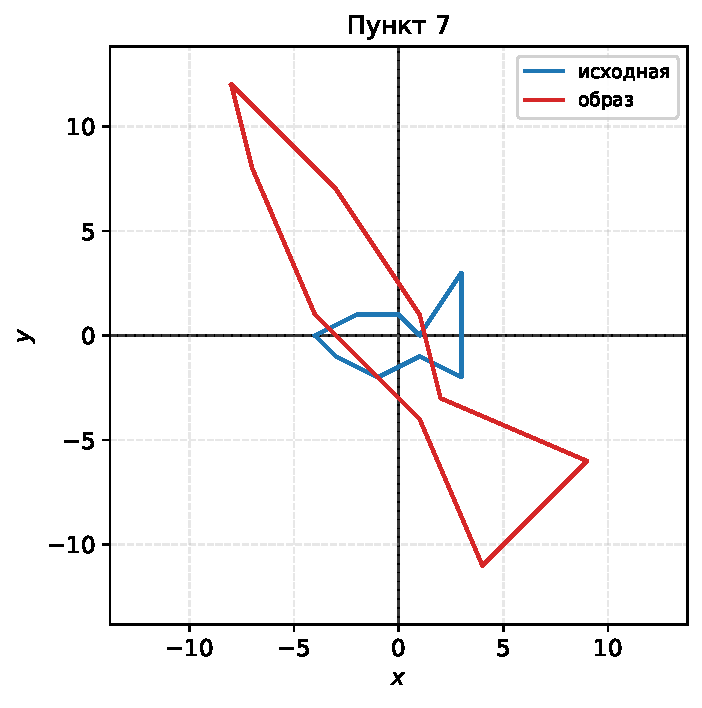
\includegraphics[width=0.55\textwidth]{../figures/p07.pdf}
\caption{Отображение пункта 7: исходный и отображённый многоугольник}
\label{fig:p07}
\end{figure}

\textbf{Анализ (задание 2).}

\emph{Определитель, ядро и образ:} \(\det A = 5\). Так как определитель
не равен нулю, отображение невырождено. Ядро:
\(\ker A = \{ \mathbf{0} \}\). Образ:
\(\operatorname{Im} A = \mathbb{R}^2\).

\emph{Собственные числа:} Характеристический многочлен:
\begin{center}\adjustbox{max width=\linewidth}{$\displaystyle \det(A - \lambda I) = \begin{vmatrix} 2 - \lambda & 1 \\ -3 & 1 - \lambda \end{vmatrix} = (2 - \lambda)(1 - \lambda) + 3 = \lambda^2 - 3\lambda + 5$}\end{center}
Корни уравнения \(\lambda^2 - 3\lambda + 5 = 0\):
\begin{center}\adjustbox{max width=\linewidth}{$\displaystyle \lambda_{1,2} = \frac{3 \pm \sqrt{9 - 20}}{2} = \frac{3 \pm i\sqrt{11}}{2}$}\end{center}
Собственные числа являются комплексно-сопряжёнными, вещественных
собственных векторов не существует.

\textbf{Вывод.}

Матрица \(A\) удовлетворяет условию, так как вектор направления прямой
\(y = 3x\), равный \(\begin{bmatrix} 1 \\ 3 \end{bmatrix}\), переходит в
\(\begin{bmatrix} 5 \\ 0 \end{bmatrix}\) (на ось \(Ox\)), а вектор
направления прямой \(y = -2x\), равный
\(\begin{bmatrix} 1 \\ -2 \end{bmatrix}\), переходит в
\(\begin{bmatrix} 0 \\ -5 \end{bmatrix}\) (на ось \(Oy\)).

Определитель \(\det A = 5 > 0\), что означает сохранение ориентации
плоскости. Модуль определителя \(|\det A| = 5\) показывает, что площадь
любого многоугольника при данном отображении увеличивается в 5 раз.
Отсутствие вещественных собственных чисел и векторов означает, что у
данного преобразования нет инвариантных прямых: оно сочетает в себе
поворот и неравномерное растяжение, не оставляя на месте ни одного
направления.

\hypertarget{ux43fux443ux43dux43aux442-8.-ux43cux435ux43dux44fux435ux442-ux43cux435ux441ux442ux430ux43cux438-y-ax-ux438-y-bx}{%
\subsection{Пункт 8. Меняет местами y = ax и y =
bx}\label{ux43fux443ux43dux43aux442-8.-ux43cux435ux43dux44fux435ux442-ux43cux435ux441ux442ux430ux43cux438-y-ax-ux438-y-bx}}

\textbf{Общий класс.}

Прямые \(y = ax\) и \(y = bx\) порождены векторами \begin{center}\adjustbox{max width=\linewidth}{$\displaystyle u_a = \begin{bmatrix} 1 \\ a \end{bmatrix},
\quad
u_b = \begin{bmatrix} 1 \\ b \end{bmatrix}$}\end{center}

Обмен прямых означает, что образ \(u_a\) лежит на прямой \(y = bx\), а
образ \(u_b\) - на прямой \(y = ax\), причём оба образа ненулевые. \begin{center}\adjustbox{max width=\linewidth}{$\displaystyle M = \begin{bmatrix} p & q \\ r & s \end{bmatrix},
\quad
M u_a = \begin{bmatrix} p + aq \\ r + as \end{bmatrix},
\quad
M u_b = \begin{bmatrix} p + bq \\ r + bs \end{bmatrix}$}\end{center}

Условие коллинеарности первого образа вектору \((1, b)^T\), а второго -
вектору \((1, a)^T\): \begin{center}\adjustbox{max width=\linewidth}{$\displaystyle r + as = b(p + aq),
\quad
r + bs = a(p + bq)$}\end{center}

Вычтем второе равенство из первого: \begin{center}\adjustbox{max width=\linewidth}{$\displaystyle (a - b)s = (b - a)p$}\end{center}

Так как \(a \neq b\), получаем \begin{center}\adjustbox{max width=\linewidth}{$\displaystyle s = -p$}\end{center}

Подставим \(s = -p\) в первое равенство: \begin{center}\adjustbox{max width=\linewidth}{$\displaystyle r - ap = bp + abq
\quad \Longrightarrow \quad
r = (a + b)p + abq$}\end{center}

Итак, общий вид матрицы: \begin{center}\adjustbox{max width=\linewidth}{$\displaystyle M = \begin{bmatrix} p & q \\ (a + b)p + abq & -p \end{bmatrix}$}\end{center}

Для такой матрицы \begin{center}\adjustbox{max width=\linewidth}{$\displaystyle M u_a = (p + aq)\,u_b,
\quad
M u_b = (p + bq)\,u_a$}\end{center}

Следовательно, обмен прямых происходит при \begin{center}\adjustbox{max width=\linewidth}{$\displaystyle p + aq \neq 0,
\quad
p + bq \neq 0$}\end{center}

Определитель: \begin{center}\adjustbox{max width=\linewidth}{$\displaystyle \det M = -p^2 - q\bigl((a + b)p + abq\bigr)
= -\bigl(p^2 + (a + b)pq + abq^2\bigr)
= -(p + aq)(p + bq)$}\end{center}

При \(a = 3\), \(b = -2\) имеем \(a + b = 1\), \(ab = -6\), поэтому \begin{center}\adjustbox{max width=\linewidth}{$\displaystyle M = \begin{bmatrix} p & q \\ p - 6q & -p \end{bmatrix},
\quad
\det M = -(p + 3q)(p - 2q)$}\end{center}

\textbf{Выбранная матрица.}

Возьмём \(p = 1\), \(q = 0\): \begin{center}\adjustbox{max width=\linewidth}{$\displaystyle A = \begin{bmatrix} 1 & 0 \\ 1 & -1 \end{bmatrix},
\quad
\det A = -1 \neq 0$}\end{center}

Проверка условия пункта: \begin{center}\adjustbox{max width=\linewidth}{$\displaystyle A \begin{bmatrix} 1 \\ 3 \end{bmatrix}
= \begin{bmatrix} 1 \\ -2 \end{bmatrix},
\quad
A \begin{bmatrix} 1 \\ -2 \end{bmatrix}
= \begin{bmatrix} 1 \\ 3 \end{bmatrix}$}\end{center}

То есть прямая \(y = 3x\) переходит в \(y = -2x\), и наоборот.

\textbf{Визуализация.}

\begin{figure}[H]
\centering
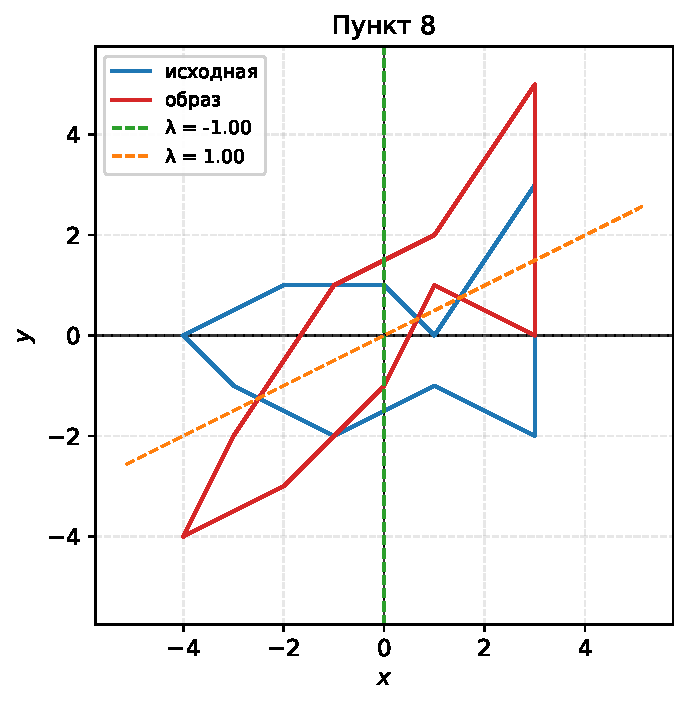
\includegraphics[width=0.55\textwidth]{../figures/p08.pdf}
\caption{Отображение пункта 8: исходный и отображённый многоугольник}
\label{fig:p08}
\end{figure}

\textbf{Анализ (задание 2).}

Определитель, ядро и образ: \(\det A = -1 \neq 0\), поэтому отображение
невырождено: \begin{center}\adjustbox{max width=\linewidth}{$\displaystyle \ker A = \{\mathbf{0}\},
\quad
\operatorname{Im} A = \mathbb{R}^2$}\end{center}

Собственные числа: \begin{center}\adjustbox{max width=\linewidth}{$\displaystyle \det(A - \lambda E)
= \begin{vmatrix} 1 - \lambda & 0 \\ 1 & -1 - \lambda \end{vmatrix}
= (1 - \lambda)(-1 - \lambda)
= \lambda^2 - 1$}\end{center}

Отсюда \(\lambda^2 - 1 = 0\), то есть \begin{center}\adjustbox{max width=\linewidth}{$\displaystyle \lambda_1 = 1,
\quad
\lambda_2 = -1$}\end{center}

Собственные векторы: Для \(\lambda_1 = 1\): \begin{center}\adjustbox{max width=\linewidth}{$\displaystyle (A - E)v =
\begin{bmatrix} 0 & 0 \\ 1 & -2 \end{bmatrix}
\begin{bmatrix} x \\ y \end{bmatrix}
= 0
\quad \Longrightarrow \quad
x - 2y = 0$}\end{center}

Собственный вектор и собственная прямая: \begin{center}\adjustbox{max width=\linewidth}{$\displaystyle v_1 = \begin{bmatrix} 2 \\ 1 \end{bmatrix},
\quad
y = \tfrac{1}{2}x$}\end{center}

Для \(\lambda_2 = -1\): \begin{center}\adjustbox{max width=\linewidth}{$\displaystyle (A + E)v =
\begin{bmatrix} 2 & 0 \\ 1 & 0 \end{bmatrix}
\begin{bmatrix} x \\ y \end{bmatrix}
= 0
\quad \Longrightarrow \quad
x = 0$}\end{center}

Собственный вектор и собственная прямая: \begin{center}\adjustbox{max width=\linewidth}{$\displaystyle v_2 = \begin{bmatrix} 0 \\ 1 \end{bmatrix},
\quad
x = 0$}\end{center}

\textbf{Вывод.}

Матрица \(A\) меняет прямые местами, потому что переводит направляющий
вектор \((1, 3)^T\) в \((1, -2)^T\) и обратно.

Отсюда же находятся собственные направления: они равны сумме и разности
направляющих векторов исходных прямых: \begin{center}\adjustbox{max width=\linewidth}{$\displaystyle A(u_a + u_b) = u_b + u_a = u_a + u_b,
\quad
A(u_a - u_b) = u_b - u_a = -(u_a - u_b)$}\end{center}

Подставляя \(u_a = (1, 3)^T\) и \(u_b = (1, -2)^T\), получаем \begin{center}\adjustbox{max width=\linewidth}{$\displaystyle u_a + u_b = \begin{bmatrix} 2 \\ 1 \end{bmatrix} = v_1,
\quad
u_a - u_b = \begin{bmatrix} 0 \\ 5 \end{bmatrix} \parallel v_2$}\end{center}

Поэтому выбранное отображение - симметрия относительно прямой
\(y = \tfrac{1}{2}x\) вдоль направления \((0, 1)^T\). Первая собственная
прямая остаётся на месте, на второй меняется знак. \begin{center}\adjustbox{max width=\linewidth}{$\displaystyle A^2 =
\begin{bmatrix} 1 & 0 \\ 1 & -1 \end{bmatrix}
\begin{bmatrix} 1 & 0 \\ 1 & -1 \end{bmatrix}
= \begin{bmatrix} 1 & 0 \\ 0 & 1 \end{bmatrix} = E$}\end{center}

То есть двукратное применение возвращает плоскость в исходное состояние,
что и означает обмен двух прямых.

Определитель \(\det A = -1 < 0\) означает смену ориентации плоскости, а
\(|\det A| = 1\) - сохранение площадей.

\hypertarget{ux43fux443ux43dux43aux442-9.-ux43aux440ux443ux433-ux43fux43bux43eux449ux430ux434ux438-1-ux43aux440ux443ux433-ux43fux43bux43eux449ux430ux434ux438-c-ux43dux435ux434ux438ux430ux433ux43eux43dux430ux43bux44cux43dux430ux44f}{%
\subsection{\texorpdfstring{Пункт 9. Круг площади 1 → круг площади \(c\)
(недиагональная)}{Пункт 9. Круг площади 1 → круг площади c (недиагональная)}}\label{ux43fux443ux43dux43aux442-9.-ux43aux440ux443ux433-ux43fux43bux43eux449ux430ux434ux438-1-ux43aux440ux443ux433-ux43fux43bux43eux449ux430ux434ux438-c-ux43dux435ux434ux438ux430ux433ux43eux43dux430ux43bux44cux43dux430ux44f}}

\textbf{Общий класс и теоретическое обоснование.}\\
Для линейного отображения \(x\mapsto Ax\) образом круга является эллипс,
полуоси которого равны сингулярным числам \(A\). Образ --- снова круг
тогда и только тогда, когда все сингулярные числа равны, то есть \begin{center}\adjustbox{max width=\linewidth}{$\displaystyle A^TA=k^2I,\qquad k>0.$}\end{center} В \(\mathbb R^2\) это означает \begin{center}\adjustbox{max width=\linewidth}{$\displaystyle A=kQ,$}\end{center} где \(Q\) --- ортогональная матрица. Ортогональная матрица в
\(\mathbb R^2\) --- это либо поворот \(R_\theta\), либо отражение.
Площадь образа умножается на \begin{center}\adjustbox{max width=\linewidth}{$\displaystyle |\det A|=k^2.$}\end{center} Чтобы круг единичной площади перешёл в круг площади \(c\), нужно
\(k=\sqrt c\). Чтобы матрица была недиагональной, нужно \(Q\ne I\),
\(Q\ne -I\) и \(Q\) не диагональное отражение. При \(c=4\) выбран
\(\theta=30^\circ\), то есть \begin{center}\adjustbox{max width=\linewidth}{$\displaystyle A=\sqrt{4}\,R_{30^\circ}=2R_{30^\circ}.$}\end{center}

\textbf{Расчёты для выбранной матрицы.} \begin{center}\adjustbox{max width=\linewidth}{$\displaystyle A_9=2R_{30^\circ}
=2\begin{pmatrix}
\cos30^\circ&-\sin30^\circ\\
\sin30^\circ&\cos30^\circ
\end{pmatrix}
=
\begin{pmatrix}
\sqrt3&-1\\
1&\sqrt3
\end{pmatrix},
\qquad
\det A_9=3+1=4=c.$}\end{center} Тогда \begin{center}\adjustbox{max width=\linewidth}{$\displaystyle A_9^TA_9=4I,$}\end{center} поэтому образом круга действительно является круг. Площадь образа: \begin{center}\adjustbox{max width=\linewidth}{$\displaystyle S_{\text{обр}}=|\det A_9|\cdot 1=4.$}\end{center} Ядро и образ: \begin{center}\adjustbox{max width=\linewidth}{$\displaystyle \det A_9=4\ne0
\quad\Longrightarrow\quad
\ker A_9=\{0\},\qquad
\operatorname{Im}A_9=\mathbb R^2.$}\end{center} Собственные числа: \begin{center}\adjustbox{max width=\linewidth}{$\displaystyle \det(A_9-\lambda I)=(\sqrt3-\lambda)^2+1
=\lambda^2-2\sqrt3\,\lambda+4,$}\end{center} \begin{center}\adjustbox{max width=\linewidth}{$\displaystyle \lambda_{1,2}=\sqrt3\pm i.$}\end{center} Вещественных собственных чисел и вещественных собственных векторов
нет.

\textbf{Выбранная матрица.} \begin{center}\adjustbox{max width=\linewidth}{$\displaystyle A_9=
\begin{pmatrix}
\sqrt3&-1\\
1&\sqrt3
\end{pmatrix}
\approx
\begin{pmatrix}
1.732&-1\\
1&1.732
\end{pmatrix}.$}\end{center}

\textbf{Визуализация.}\\
Образ многоугольника и образ круга единичной площади (радиуса
\(1/\sqrt\pi\)) показаны на рисунках~\ref{fig:p09} и p09c: круг переходит в круг
площади \(4\), повёрнутый на \(30^\circ\).

\begin{figure}[H]
\centering
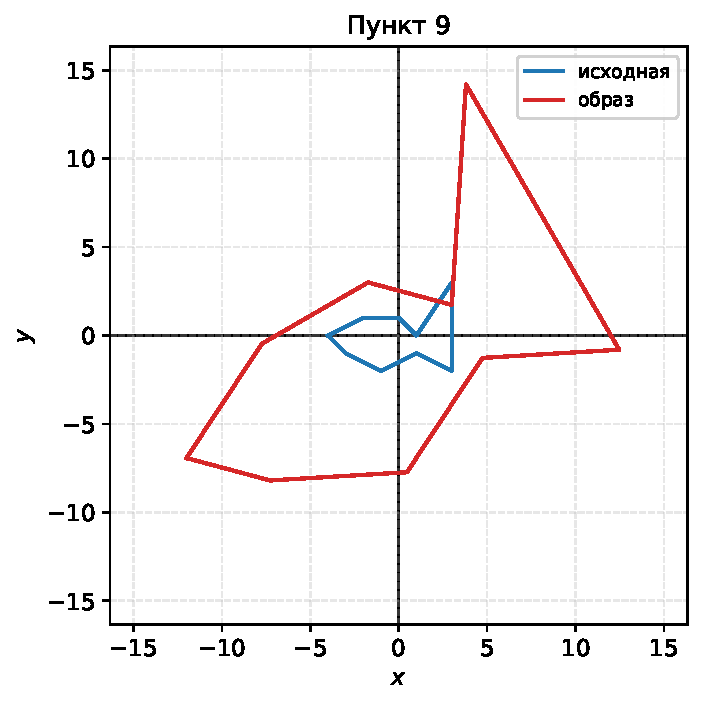
\includegraphics[width=0.55\textwidth]{../figures/p09.pdf}
\caption{Пункт 9: образ многоугольника}
\label{fig:p09}
\end{figure}

\begin{figure}[H]
\centering
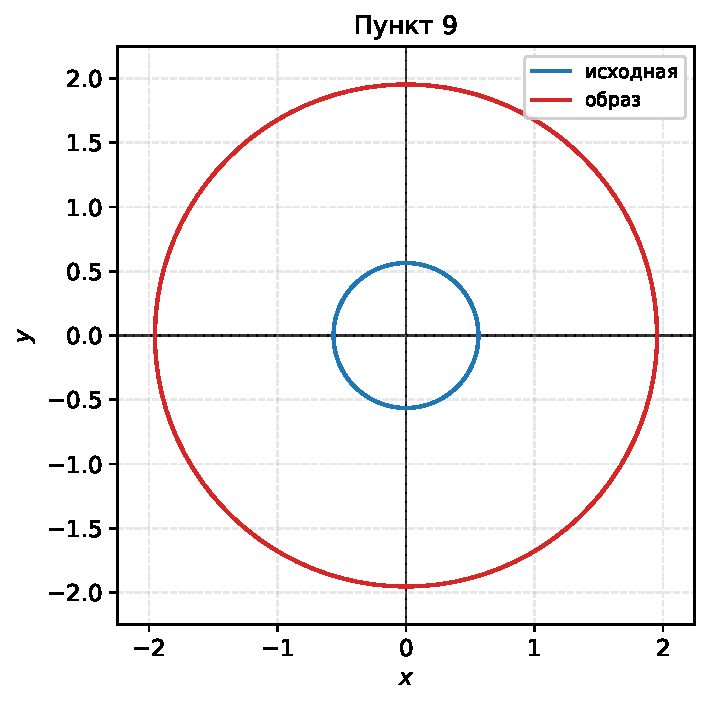
\includegraphics[width=0.55\textwidth]{../figures/p09c.pdf}
\caption{Пункт 9: круг единичной площади и его образ}
\label{fig:p09c}
\end{figure}

\textbf{Вывод.}\\
\(A_9\) --- недиагональная матрица подобия: растяжение в \(2\) раза и
поворот на \(30^\circ\). Она переводит круг единичной площади в круг
площади \(4\).

\begin{center}\rule{0.5\linewidth}{0.5pt}\end{center}

\hypertarget{ux43fux443ux43dux43aux442-10.-ux43aux440ux443ux433-ux43fux43bux43eux449ux430ux434ux438-1-ux43dux435ux43aux440ux443ux433-ux43fux43bux43eux449ux430ux434ux438-d-ux43dux435ux434ux438ux430ux433ux43eux43dux430ux43bux44cux43dux430ux44f}{%
\subsection{\texorpdfstring{Пункт 10. Круг площади 1 → некруг площади
\(d\)
(недиагональная)}{Пункт 10. Круг площади 1 → некруг площади d (недиагональная)}}\label{ux43fux443ux43dux43aux442-10.-ux43aux440ux443ux433-ux43fux43bux43eux449ux430ux434ux438-1-ux43dux435ux43aux440ux443ux433-ux43fux43bux43eux449ux430ux434ux438-d-ux43dux435ux434ux438ux430ux433ux43eux43dux430ux43bux44cux43dux430ux44f}}

\textbf{Общий класс и теоретическое обоснование.}\\
Нужны недиагональные матрицы \(A\), для которых образом круга является
эллипс, а не круг. Это равносильно тому, что сингулярные числа различны,
то есть \begin{center}\adjustbox{max width=\linewidth}{$\displaystyle A^TA\ne k^2I.$}\end{center} Площадь образа равна \begin{center}\adjustbox{max width=\linewidth}{$\displaystyle |\det A|.$}\end{center} Поэтому общий класс: \begin{center}\adjustbox{max width=\linewidth}{$\displaystyle |\det A|=d,
\qquad
A^TA\ne k^2I,
\qquad
A \text{ недиагональна}.$}\end{center} При \(d=14\) выбрана верхнетреугольная матрица с разными
диагональными элементами.

\textbf{Расчёты для выбранной матрицы.} \begin{center}\adjustbox{max width=\linewidth}{$\displaystyle A_{10}=
\begin{pmatrix}
14&8\\
0&1
\end{pmatrix},
\qquad
\det A_{10}=14=d.$}\end{center} Ядро и образ: \begin{center}\adjustbox{max width=\linewidth}{$\displaystyle \det A_{10}=14\ne0
\quad\Longrightarrow\quad
\ker A_{10}=\{0\},\qquad
\operatorname{Im}A_{10}=\mathbb R^2.$}\end{center} Собственные числа --- диагональные элементы: \begin{center}\adjustbox{max width=\linewidth}{$\displaystyle \lambda_1=14,\qquad \lambda_2=1.$}\end{center} Собственные векторы: \begin{center}\adjustbox{max width=\linewidth}{$\displaystyle \lambda=14:\quad
(A_{10}-14I)v=0
\;\Longrightarrow\;
\begin{pmatrix}0&8\\0&-13\end{pmatrix}v=0
\;\Longrightarrow\;
v=(1,0);$}\end{center} \begin{center}\adjustbox{max width=\linewidth}{$\displaystyle \lambda=1:\quad
(A_{10}-I)v=0
\;\Longrightarrow\;
\begin{pmatrix}13&8\\0&0\end{pmatrix}v=0
\;\Longrightarrow\;
13x+8y=0
\;\Longrightarrow\;
v=(8,-13).$}\end{center} Проверка, что образ --- не круг: \begin{center}\adjustbox{max width=\linewidth}{$\displaystyle A_{10}^TA_{10}=
\begin{pmatrix}
196&112\\
112&65
\end{pmatrix}.$}\end{center} Её собственные значения --- корни \(\mu^2-261\mu+196=0\): \begin{center}\adjustbox{max width=\linewidth}{$\displaystyle \mu_{1,2}=\frac{261\pm\sqrt{67337}}{2},\qquad \mu_1\approx260.25,\quad \mu_2\approx0.753,$}\end{center} они различны, поэтому сингулярные числа \begin{center}\adjustbox{max width=\linewidth}{$\displaystyle \sigma_1=\sqrt{\mu_1}\approx16.13,\qquad \sigma_2=\sqrt{\mu_2}\approx0.868$}\end{center} различны. Значит, образом круга является эллипс, а не круг. Площадь:
\begin{center}\adjustbox{max width=\linewidth}{$\displaystyle |\det A_{10}|=\sigma_1\sigma_2=\sqrt{196}=14.$}\end{center}

\textbf{Выбранная матрица.} \begin{center}\adjustbox{max width=\linewidth}{$\displaystyle A_{10}=
\begin{pmatrix}
14&8\\
0&1
\end{pmatrix}.$}\end{center}

\textbf{Визуализация.}\\
Образ многоугольника и образ круга единичной площади показаны на
рисунках~\ref{fig:p10} и p10c.

\begin{figure}[H]
\centering
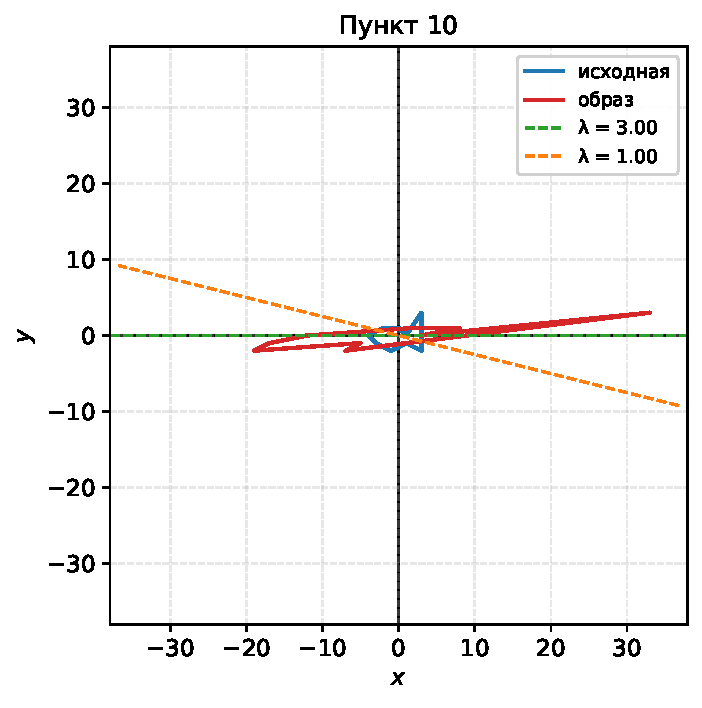
\includegraphics[width=0.55\textwidth]{../figures/p10.pdf}
\caption{Пункт 10: образ многоугольника}
\label{fig:p10}
\end{figure}

\begin{figure}[H]
\centering
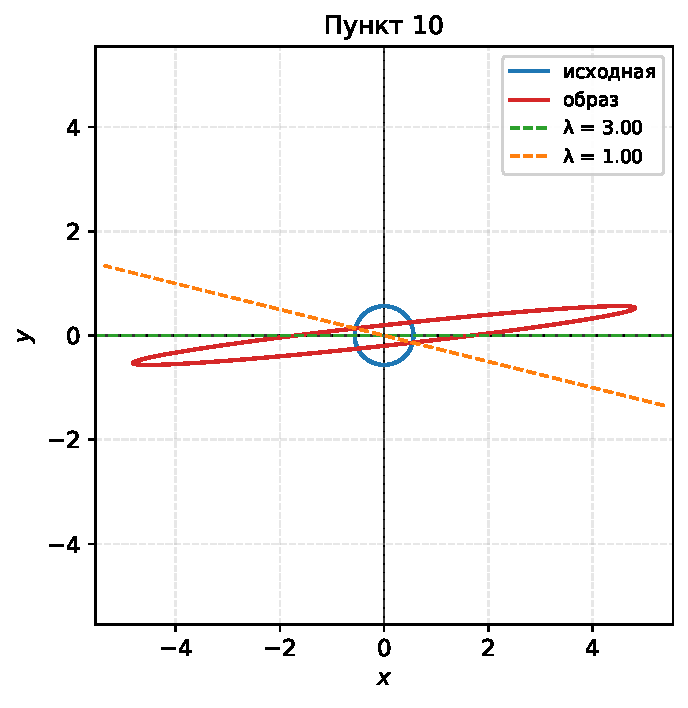
\includegraphics[width=0.55\textwidth]{../figures/p10c.pdf}
\caption{Пункт 10: круг единичной площади и его образ}
\label{fig:p10c}
\end{figure}

\textbf{Вывод.}\\
\(A_{10}\) недиагональна, \(|\det A_{10}|=14\), сингулярные числа
различны. Поэтому круг единичной площади переходит в эллипс площади
\(14\), а не в круг.

\begin{center}\rule{0.5\linewidth}{0.5pt}\end{center}

\hypertarget{ux43fux443ux43dux43aux442-11.-ux43fux435ux440ux43fux435ux43dux434ux438ux43aux443ux43bux44fux440ux43dux44bux435-ux441ux43eux431ux441ux442ux432ux435ux43dux43dux44bux435-ux432ux435ux43aux442ux43eux440ux44b-ux43dux435-ux43dux430-y-0-ux438-y-x}{%
\subsection{Пункт 11. Перпендикулярные собственные векторы не на y = 0 и
y =
x}\label{ux43fux443ux43dux43aux442-11.-ux43fux435ux440ux43fux435ux43dux434ux438ux43aux443ux43bux44fux440ux43dux44bux435-ux441ux43eux431ux441ux442ux432ux435ux43dux43dux44bux435-ux432ux435ux43aux442ux43eux440ux44b-ux43dux435-ux43dux430-y-0-ux438-y-x}}

\textbf{Общий класс.}

Вещественная матрица \(2 \times 2\) имеет ортогональные собственные
векторы тогда и только тогда, когда она является симметричной (случай
кратной единичной матрицы \(cI\) отпадает, так как для неё собственными
являются любые векторы, в том числе лежащие на \(y=0\) и \(y=x\)).

Пусть матрица имеет вид
\begin{center}\adjustbox{max width=\linewidth}{$\displaystyle M = \begin{bmatrix} p & q \\ q & r \end{bmatrix}$}\end{center}

Проверим условия на собственные векторы: 1. Если собственный вектор
лежит на прямой \(y = 0\), он коллинеарен
\(\begin{bmatrix} 1 \\ 0 \end{bmatrix}\). Тогда
\(M \begin{bmatrix} 1 \\ 0 \end{bmatrix} = \begin{bmatrix} p \\ q \end{bmatrix} = \lambda \begin{bmatrix} 1 \\ 0 \end{bmatrix}\),
откуда следует \(q = 0\). Чтобы исключить этот случай, потребуем
\(q \neq 0\). 2. Если собственный вектор лежит на прямой \(y = x\), он
коллинеарен \(\begin{bmatrix} 1 \\ 1 \end{bmatrix}\). Тогда
\(M \begin{bmatrix} 1 \\ 1 \end{bmatrix} = \begin{bmatrix} p+q \\ q+r \end{bmatrix} = \lambda \begin{bmatrix} 1 \\ 1 \end{bmatrix}\),
откуда \(p+q = q+r \implies p = r\). Чтобы исключить этот случай,
потребуем \(p \neq r\).

Таким образом, общий класс матриц:
\begin{center}\adjustbox{max width=\linewidth}{$\displaystyle M = \begin{bmatrix} p & q \\ q & r \end{bmatrix}, \quad q \neq 0, \quad p \neq r$}\end{center}

\textbf{Выбранная матрица.}

Возьмём простейшие целые значения, удовлетворяющие условиям, например,
\(p = 2\), \(q = 1\), \(r = 0\):
\begin{center}\adjustbox{max width=\linewidth}{$\displaystyle A = \begin{bmatrix} 2 & 1 \\ 1 & 0 \end{bmatrix}$}\end{center}

\textbf{Визуализация.}

\begin{figure}[H]
\centering
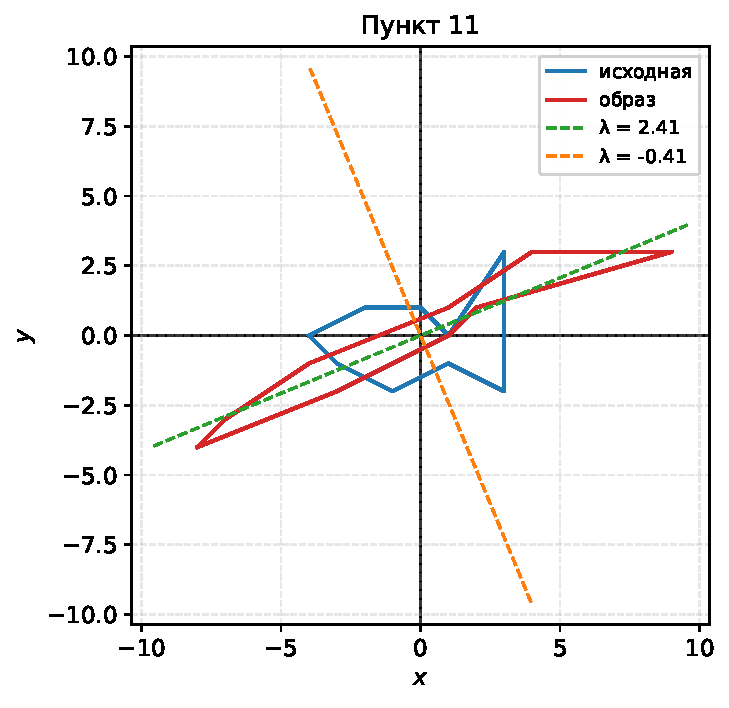
\includegraphics[width=0.55\textwidth]{../figures/p11.pdf}
\caption{Отображение пункта 11: исходный и отображённый многоугольник}
\label{fig:p11}
\end{figure}

\textbf{Анализ (задание 2).}

Характеристический многочлен:
\begin{center}\adjustbox{max width=\linewidth}{$\displaystyle \det(A - \lambda I) = \begin{vmatrix} 2 - \lambda & 1 \\ 1 & -\lambda \end{vmatrix} = (2 - \lambda)(-\lambda) - 1 = \lambda^2 - 2\lambda - 1$}\end{center}

Корни уравнения \(\lambda^2 - 2\lambda - 1 = 0\):
\begin{center}\adjustbox{max width=\linewidth}{$\displaystyle \lambda_{1,2} = \frac{2 \pm \sqrt{4 - 4(-1)}}{2} = 1 \pm \sqrt{2}$}\end{center}

Для \(\lambda_1 = 1 + \sqrt{2}\) решаем систему
\((A - \lambda_1 I)v = 0\):
\begin{center}\adjustbox{max width=\linewidth}{$\displaystyle (2 - (1 + \sqrt{2}))x + y = 0 \implies (1 - \sqrt{2})x + y = 0 \implies y = (\sqrt{2} - 1)x$}\end{center}

Собственный вектор:
\begin{center}\adjustbox{max width=\linewidth}{$\displaystyle v_1 = \begin{bmatrix} 1 \\ \sqrt{2} - 1 \end{bmatrix}$}\end{center}

Для \(\lambda_2 = 1 - \sqrt{2}\):
\begin{center}\adjustbox{max width=\linewidth}{$\displaystyle (2 - (1 - \sqrt{2}))x + y = 0 \implies (1 + \sqrt{2})x + y = 0 \implies y = -(1 + \sqrt{2})x$}\end{center}

Собственный вектор:
\begin{center}\adjustbox{max width=\linewidth}{$\displaystyle v_2 = \begin{bmatrix} 1 \\ -1 - \sqrt{2} \end{bmatrix}$}\end{center}

Скалярное произведение:
\begin{center}\adjustbox{max width=\linewidth}{$\displaystyle v_1 \cdot v_2 = 1 \cdot 1 + (\sqrt{2} - 1)(-1 - \sqrt{2}) = 1 - (\sqrt{2} - 1)(\sqrt{2} + 1) = 1 - (2 - 1) = 0$}\end{center}

Векторы перпендикулярны.

Отношение координат для \(v_1\):
\begin{center}\adjustbox{max width=\linewidth}{$\displaystyle y/x = \sqrt{2} - 1 \approx 0.414 \neq 0 \quad и \neq 1$}\end{center}

Отношение координат для \(v_2\):
\begin{center}\adjustbox{max width=\linewidth}{$\displaystyle y/x = -1 - \sqrt{2} \approx -2.414 \neq 0 \quad и \neq 1$}\end{center}

Ни один из векторов не лежит на прямых \(y = 0\) и \(y = x\).

\textbf{Вывод.}

Матрица \(A\) является симметричной, что по спектральной теореме
гарантирует вещественность собственных чисел и ортогональность
собственных векторов. Наложенные ограничения \(q \neq 0\) и \(p \neq r\)
геометрически означают, что главные оси растяжения (собственные
направления) не совпадают с осями координат (\(y=0\)) и биссектрисой
первого координатного угла (\(y=x\)). Выбранная матрица полностью
удовлетворяет всем условиям пункта.

\hypertarget{ux43fux443ux43dux43aux442-12.-ux43dux435ux442-ux434ux432ux443ux445-ux43dux435ux43aux43eux43bux43bux438ux43dux435ux430ux440ux43dux44bux445-ux441ux43eux431ux441ux442ux432ux435ux43dux43dux44bux445-ux432ux435ux43aux442ux43eux440ux43eux432}{%
\subsection{Пункт 12. Нет двух неколлинеарных собственных
векторов}\label{ux43fux443ux43dux43aux442-12.-ux43dux435ux442-ux434ux432ux443ux445-ux43dux435ux43aux43eux43bux43bux438ux43dux435ux430ux440ux43dux44bux445-ux441ux43eux431ux441ux442ux432ux435ux43dux43dux44bux445-ux432ux435ux43aux442ux43eux440ux43eux432}}

\textbf{Общий класс.}

Матрица \(2 \times 2\) имеет два неколлинеарных собственных вектора
тогда и только тогда, когда она диагонализуема над \(\mathbb{R}\). Чтобы
у отображения \emph{не было} двух неколлинеарных собственных векторов,
матрица должна иметь ровно одно собственное направление.

Это возможно только в том случае, если у матрицы есть единственное
вещественное собственное число \(\lambda\) алгебраической кратности 2,
но геометрической кратности 1. Такие матрицы не диагонализуемы и подобны
жордановой клетке. В базисе, содержащем этот единственный собственный
вектор, общий класс таких матриц имеет верхнетреугольный вид
\begin{center}\adjustbox{max width=\linewidth}{$\displaystyle M = \begin{bmatrix} \lambda & k \\ 0 & \lambda \end{bmatrix}, \quad \lambda \in \mathbb{R}, \; k \neq 0$}\end{center}

\textbf{Выбранная матрица.}

Возьмём простейшие значения \(\lambda = 2\) и \(k = 1\)
\begin{center}\adjustbox{max width=\linewidth}{$\displaystyle A = \begin{bmatrix} 2 & 1 \\ 0 & 2 \end{bmatrix}$}\end{center}

\textbf{Визуализация.}

\begin{figure}[H]
\centering
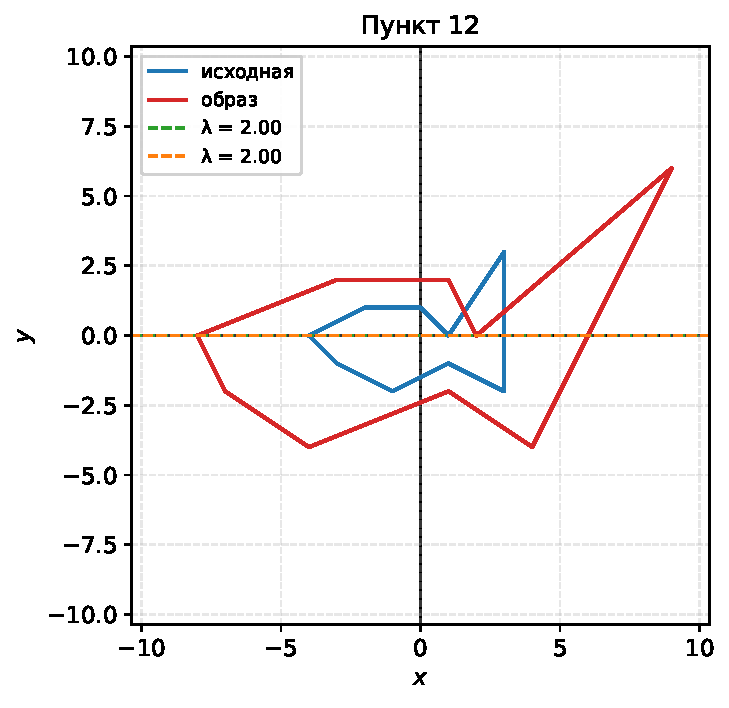
\includegraphics[width=0.55\textwidth]{../figures/p12.pdf}
\caption{Отображение пункта 12: исходный и отображённый многоугольник}
\label{fig:p12}
\end{figure}

\textbf{Анализ (задание 2).}

Характеристический многочлен:
\begin{center}\adjustbox{max width=\linewidth}{$\displaystyle \det(A - \mu I) = \begin{vmatrix} 2 - \mu & 1 \\ 0 & 2 - \mu \end{vmatrix} = (2 - \mu)^2 = 0$}\end{center}

Матрица имеет единственное собственное число \(\mu = 2\) алгебраической
кратности 2.

Для нахождения собственных векторов решаем систему \((A - 2I)v = 0\):
\begin{center}\adjustbox{max width=\linewidth}{$\displaystyle \begin{bmatrix} 0 & 1 \\ 0 & 0 \end{bmatrix} \begin{bmatrix} x \\ y \end{bmatrix} = \begin{bmatrix} 0 \\ 0 \end{bmatrix}$}\end{center}

Это уравнение сводится к единственному условию \(y = 0\). Переменная
\(x\) остаётся свободной. Следовательно, существует только одно
собственное направление, а собственный вектор (с точностью до скалярного
множителя) единственный: \begin{center}\adjustbox{max width=\linewidth}{$\displaystyle v = \begin{bmatrix} 1 \\ 0 \end{bmatrix}$}\end{center}

Геометрическая кратность собственного числа равна 1, что строго меньше
его алгебраической кратности (2).

\textbf{Вывод.}

Матрица \(A\) является жордановой клеткой размера 2. Наличие
единственного собственного вектора \(v = (1, 0)^T\) означает, что
преобразование имеет только одну инвариантную прямую (ось \(Ox\)). Вдоль
этой прямой происходит чистое растяжение в \(\lambda = 2\) раза.

Во всех остальных направлениях преобразование не просто масштабирует
векторы, но и ``сдвигает'' их вдоль инвариантной прямой (добавляет к
координате \(x\) компоненту, пропорциональную \(y\)). Геометрически это
классический косой сдвиг. Поскольку геометрическая кратность
собственного числа (1) меньше его алгебраической кратности (2), матрица
не может быть приведена к диагональному виду, что и гарантирует
отсутствие второго неколлинеарного собственного вектора.

\hypertarget{ux43fux443ux43dux43aux442-13.-ux43dux435ux442-ux432ux435ux449ux435ux441ux442ux432ux435ux43dux43dux44bux445-ux441ux43eux431ux441ux442ux432ux435ux43dux43dux44bux445-ux432ux435ux43aux442ux43eux440ux43eux432}{%
\subsection{Пункт 13. Нет вещественных собственных
векторов}\label{ux43fux443ux43dux43aux442-13.-ux43dux435ux442-ux432ux435ux449ux435ux441ux442ux432ux435ux43dux43dux44bux445-ux441ux43eux431ux441ux442ux432ux435ux43dux43dux44bux445-ux432ux435ux43aux442ux43eux440ux43eux432}}

\textbf{Общий класс и теоретическое обоснование.}\\
Для вещественной матрицы \(2\times2\) \begin{center}\adjustbox{max width=\linewidth}{$\displaystyle A=\begin{pmatrix}a&b\\c&d\end{pmatrix}$}\end{center} отсутствие вещественных собственных чисел равносильно отрицательности
дискриминанта характеристического многочлена: \begin{center}\adjustbox{max width=\linewidth}{$\displaystyle (\operatorname{tr}A)^2-4\det A<0.$}\end{center} В этом случае собственные числа комплексно-сопряжённые
\(\alpha\pm i\beta\), \(\beta\ne0\), и вещественных собственных векторов
нет. Частный удобный класс --- матрицы поворота с растяжением: \begin{center}\adjustbox{max width=\linewidth}{$\displaystyle A=\alpha I+\beta J,\qquad
J=\begin{pmatrix}0&-1\\1&0\end{pmatrix},\quad \beta\ne0.$}\end{center} В коде выбран чистый поворот на \(90^\circ\).

\textbf{Расчёты для выбранной матрицы.} \begin{center}\adjustbox{max width=\linewidth}{$\displaystyle A_{13}=
\begin{pmatrix}
0&-1\\
1&0
\end{pmatrix}=R_{90^\circ}.$}\end{center} \begin{center}\adjustbox{max width=\linewidth}{$\displaystyle \det A_{13}=1\ne0
\quad\Longrightarrow\quad
\ker A_{13}=\{0\},\qquad
\operatorname{Im}A_{13}=\mathbb R^2.$}\end{center} Характеристический многочлен: \begin{center}\adjustbox{max width=\linewidth}{$\displaystyle \det(A_{13}-\lambda I)=\lambda^2+1.$}\end{center} Вещественных собственных чисел нет. Комплексные: \begin{center}\adjustbox{max width=\linewidth}{$\displaystyle \lambda_{1,2}=\pm i,
\qquad
v_i=(1,-i),\quad v_{-i}=(1,i).$}\end{center} Следовательно, вещественных собственных векторов нет.

\textbf{Выбранная матрица.} \begin{center}\adjustbox{max width=\linewidth}{$\displaystyle A_{13}=
\begin{pmatrix}
0&-1\\
1&0
\end{pmatrix}.$}\end{center}

\textbf{Визуализация.}

\begin{figure}[H]
\centering
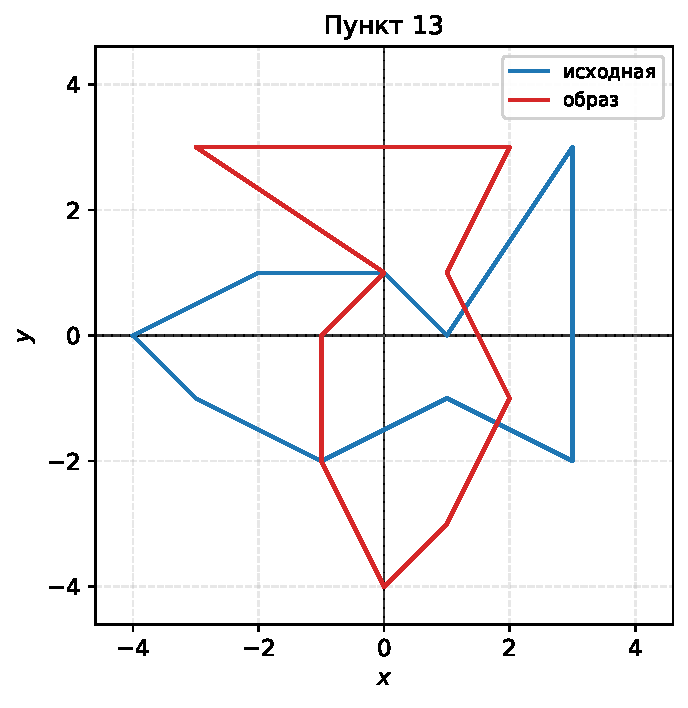
\includegraphics[width=0.55\textwidth]{../figures/p13.pdf}
\caption{Пункт 13: отображение без вещественных собственных векторов}
\label{fig:p13}
\end{figure}

Круг переходит в такой же круг, повёрнутый на \(90^\circ\).

\textbf{Вывод.}\\
\(A_{13}\) --- вещественная матрица без вещественных собственных
векторов. Она ортогональна, но не инволютивна: \begin{center}\adjustbox{max width=\linewidth}{$\displaystyle A_{13}^TA_{13}=I,\qquad A_{13}^2=-I\ne I.$}\end{center}

\begin{center}\rule{0.5\linewidth}{0.5pt}\end{center}

\hypertarget{ux43fux443ux43dux43aux442-14.-ux43bux44eux431ux43eux439-ux43dux435ux43dux443ux43bux435ux432ux43eux439-ux432ux435ux43aux442ux43eux440-ux441ux43eux431ux441ux442ux432ux435ux43dux43dux44bux439}{%
\subsection{Пункт 14. Любой ненулевой вектор
собственный}\label{ux43fux443ux43dux43aux442-14.-ux43bux44eux431ux43eux439-ux43dux435ux43dux443ux43bux435ux432ux43eux439-ux432ux435ux43aux442ux43eux440-ux441ux43eux431ux441ux442ux432ux435ux43dux43dux44bux439}}

\textbf{Общий класс.}

Пусть для любого ненулевого вектора \(v\) выполняется условие
\(Mv = \lambda_v v\), где \(\lambda_v\) - некоторое число, зависящее от
\(v\).

Рассмотрим базисные векторы
\(e_1 = \begin{bmatrix} 1 \\ 0 \end{bmatrix}\) и
\(e_2 = \begin{bmatrix} 0 \\ 1 \end{bmatrix}\).
\begin{center}\adjustbox{max width=\linewidth}{$\displaystyle M e_1 = \lambda_1 e_1 \implies \text{первый столбец } M \text{ равен } \begin{bmatrix} \lambda_1 \\ 0 \end{bmatrix}$}\end{center}
\begin{center}\adjustbox{max width=\linewidth}{$\displaystyle M e_2 = \lambda_2 e_2 \implies \text{второй столбец } M \text{ равен } \begin{bmatrix} 0 \\ \lambda_2 \end{bmatrix}$}\end{center}

Таким образом, матрица имеет диагональный вид
\(M = \begin{bmatrix} \lambda_1 & 0 \\ 0 & \lambda_2 \end{bmatrix}\)

Теперь рассмотрим вектор \(v = \begin{bmatrix} 1 \\ 1 \end{bmatrix}\)
\begin{center}\adjustbox{max width=\linewidth}{$\displaystyle M \begin{bmatrix} 1 \\ 1 \end{bmatrix} = \begin{bmatrix} \lambda_1 \\ \lambda_2 \end{bmatrix}$}\end{center}

Чтобы этот вектор был собственным, он должен быть коллинеарен исходному
вектору \(\begin{bmatrix} 1 \\ 1 \end{bmatrix}\), что возможно только
при \(\lambda_1 = \lambda_2 = \lambda\)
\begin{center}\adjustbox{max width=\linewidth}{$\displaystyle M = \begin{bmatrix} \lambda & 0 \\ 0 & \lambda \end{bmatrix} = \lambda I, \quad \lambda \in \mathbb{R}$}\end{center}

\textbf{Выбранная матрица.}

Возьмём \(\lambda = 3\):
\begin{center}\adjustbox{max width=\linewidth}{$\displaystyle A = \begin{bmatrix} 3 & 0 \\ 0 & 3 \end{bmatrix}$}\end{center}

\textbf{Визуализация.}

\begin{figure}[H]
\centering
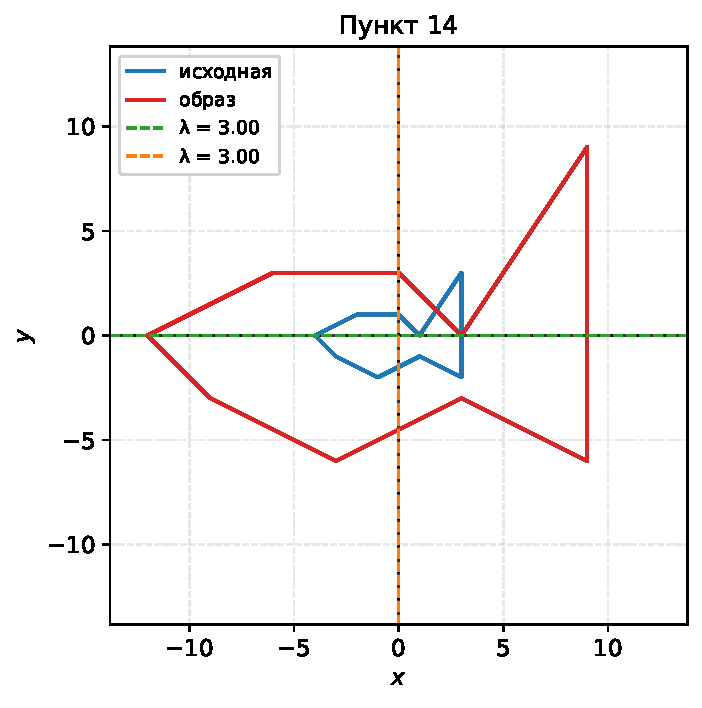
\includegraphics[width=0.55\textwidth]{../figures/p14.pdf}
\caption{Отображение пункта 14: исходный и отображённый многоугольник}
\label{fig:p14}
\end{figure}

\textbf{Анализ (задание 2).}

Определитель, ядро и образ: \begin{center}\adjustbox{max width=\linewidth}{$\displaystyle \det A = 3 \cdot 3 - 0 = 9 \neq 0$}\end{center}

Так как определитель не равен нулю, отображение невырождено.

Ядро: \(\ker A = \{\mathbf{0}\}\).

Образ: \(\operatorname{Im} A = \mathbb{R}^2\).

Характеристический многочлен:
\begin{center}\adjustbox{max width=\linewidth}{$\displaystyle \det(A - \mu I) = \begin{vmatrix} 3 - \mu & 0 \\ 0 & 3 - \mu \end{vmatrix} = (3 - \mu)^2 = 0$}\end{center}

Матрица имеет единственное собственное число \(\mu = 3\) алгебраической
кратности 2.

Для нахождения собственных векторов решаем систему \((A - 3I)v = 0\):
\begin{center}\adjustbox{max width=\linewidth}{$\displaystyle \begin{bmatrix} 0 & 0 \\ 0 & 0 \end{bmatrix} \begin{bmatrix} x \\ y \end{bmatrix} = \begin{bmatrix} 0 \\ 0 \end{bmatrix}$}\end{center}

Это тождество выполняется для любых \(x\) и \(y\). Следовательно,
геометрическая кратность собственного числа равна 2, и любой ненулевой
вектор плоскости является собственным. Базис пространства собственных
векторов можно выбрать как
\(v_1 = \begin{bmatrix} 1 \\ 0 \end{bmatrix}\) и
\(v_2 = \begin{bmatrix} 0 \\ 1 \end{bmatrix}\)

\textbf{Вывод.}

Матрица \(A = 3I\) представляет собой гомотетию (равномерное
масштабирование) плоскости с коэффициентом 3 относительно начала
координат. Поскольку преобразование просто умножает координаты любого
вектора на скаляр 3, его направление не меняется, что строго
соответствует условию: любой ненулевой вектор является собственным.

Определитель \(\det A = 9 > 0\) означает сохранение ориентации
плоскости, а \(|\det A| = 9\) показывает, что площадь любой фигуры при
данном отображении увеличивается в 9 раз (что геометрически
соответствует квадрату коэффициента масштабирования \(3^2\)). Такая
матрица является симметричной, ортогональной (с точностью до скалярного
множителя) и коммутирует с любой другой матрицей \(2 \times 2\).

\hypertarget{ux43fux443ux43dux43aux442-15.-abne-ba}{%
\subsection{\texorpdfstring{Пункт 15.
\(AB\ne BA\)}{Пункт 15. AB\textbackslash ne BA}}\label{ux43fux443ux43dux43aux442-15.-abne-ba}}

\textbf{Общий класс и теоретическое обоснование.}\\
Нужны пары матриц \(A,B\), для которых коммутатор ненулевой: \begin{center}\adjustbox{max width=\linewidth}{$\displaystyle [A,B]=AB-BA\ne0.$}\end{center} Общий класс --- все некоммутирующие пары. Простой достаточный класс
--- две верхнетреугольные матрицы с разными внедиагональными элементами.
В коде выбраны \begin{center}\adjustbox{max width=\linewidth}{$\displaystyle A=\begin{pmatrix}1&1\\0&1\end{pmatrix},
\qquad
B=\begin{pmatrix}2&1\\0&1\end{pmatrix}.$}\end{center}

\textbf{Расчёты для выбранной пары.} \begin{center}\adjustbox{max width=\linewidth}{$\displaystyle AB=
\begin{pmatrix}
1&1\\
0&1
\end{pmatrix}
\begin{pmatrix}
2&1\\
0&1
\end{pmatrix}
=
\begin{pmatrix}
2&2\\
0&1
\end{pmatrix},$}\end{center} \begin{center}\adjustbox{max width=\linewidth}{$\displaystyle BA=
\begin{pmatrix}
2&1\\
0&1
\end{pmatrix}
\begin{pmatrix}
1&1\\
0&1
\end{pmatrix}
=
\begin{pmatrix}
2&3\\
0&1
\end{pmatrix}.$}\end{center} Поэтому \begin{center}\adjustbox{max width=\linewidth}{$\displaystyle AB\ne BA.$}\end{center} Все матрицы \(A,B,AB,BA\) обратимы: \begin{center}\adjustbox{max width=\linewidth}{$\displaystyle \det A=1,\qquad \det B=2,\qquad
\det(AB)=\det(BA)=2.$}\end{center} Значит, \begin{center}\adjustbox{max width=\linewidth}{$\displaystyle \ker A=\ker B=\ker(AB)=\ker(BA)=\{0\},$}\end{center} \begin{center}\adjustbox{max width=\linewidth}{$\displaystyle \operatorname{Im}A=\operatorname{Im}B=\operatorname{Im}(AB)=\operatorname{Im}(BA)=\mathbb R^2.$}\end{center} Собственные числа и векторы: \begin{center}\adjustbox{max width=\linewidth}{$\displaystyle A:\quad \lambda=1\ \text{(кратность 2)},\quad v=(1,0);$}\end{center} \begin{center}\adjustbox{max width=\linewidth}{$\displaystyle B:\quad \lambda=2,\ v=(1,0);\qquad
\lambda=1,\ v=(1,-1);$}\end{center} \begin{center}\adjustbox{max width=\linewidth}{$\displaystyle AB:\quad \lambda=2,\ v=(1,0);\qquad
\lambda=1,\ v=(2,-1);$}\end{center} \begin{center}\adjustbox{max width=\linewidth}{$\displaystyle BA:\quad \lambda=2,\ v=(1,0);\qquad
\lambda=1,\ v=(3,-1).$}\end{center}

\textbf{Выбранные матрицы.} \begin{center}\adjustbox{max width=\linewidth}{$\displaystyle A_{15}=\begin{pmatrix}1&1\\0&1\end{pmatrix},
\qquad
B_{15}=\begin{pmatrix}2&1\\0&1\end{pmatrix}.$}\end{center}

\textbf{Визуализация.}\\
В \texttt{block\_b.py} строятся четыре картинки:

\begin{figure}[H]
\centering
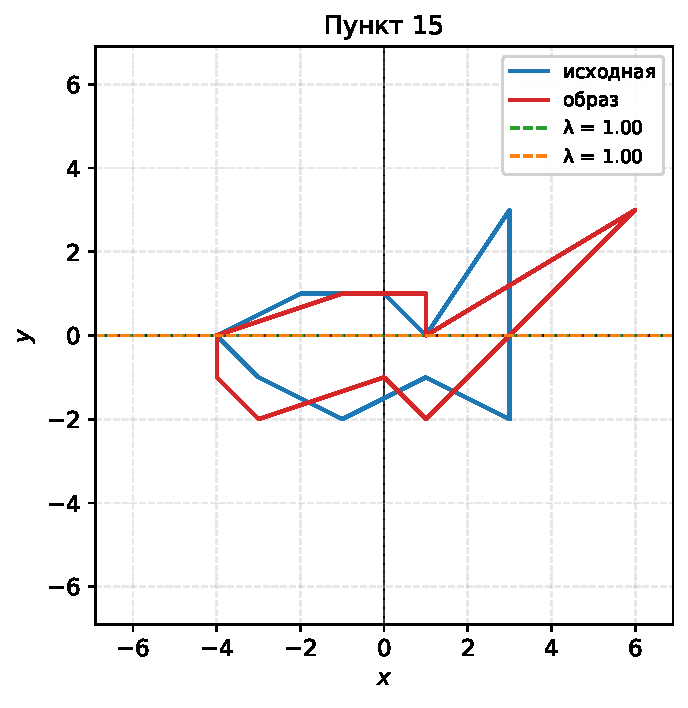
\includegraphics[width=0.55\textwidth]{../figures/p15A.pdf}
\caption{Пункт 15: отображение \(A\)}
\label{fig:p15A}
\end{figure}

\begin{figure}[H]
\centering
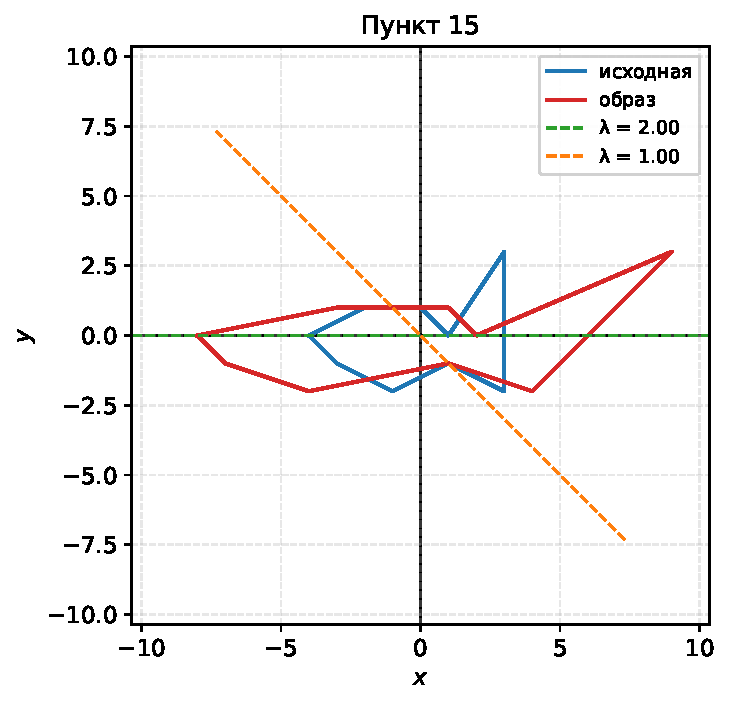
\includegraphics[width=0.55\textwidth]{../figures/p15B.pdf}
\caption{Пункт 15: отображение \(B\)}
\label{fig:p15B}
\end{figure}

\begin{figure}[H]
\centering
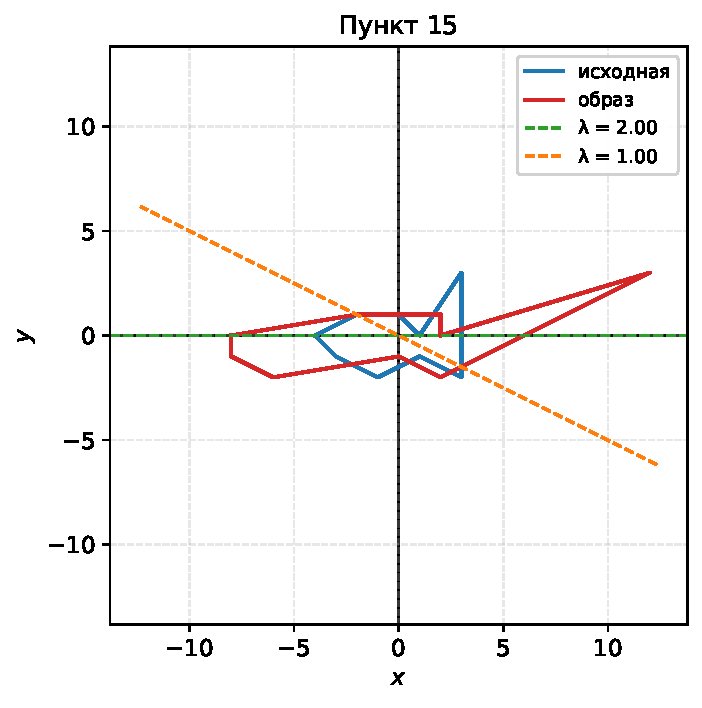
\includegraphics[width=0.55\textwidth]{../figures/p15AB.pdf}
\caption{Пункт 15: отображение \(AB\)}
\label{fig:p15AB}
\end{figure}

\begin{figure}[H]
\centering
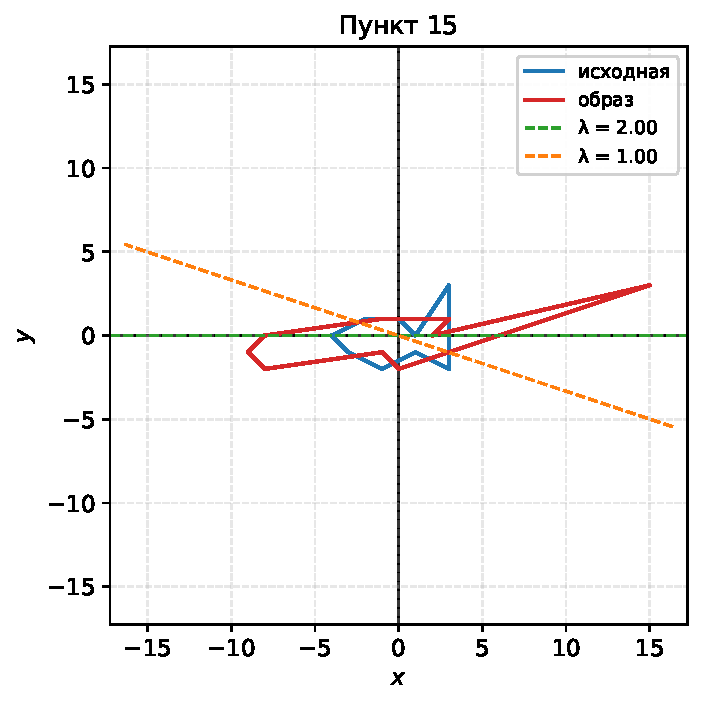
\includegraphics[width=0.55\textwidth]{../figures/p15BA.pdf}
\caption{Пункт 15: отображение \(BA\)}
\label{fig:p15BA}
\end{figure}

По ним видно, что \(AB\) и \(BA\) дают разные образы.

\textbf{Вывод.}\\
Порядок применения отображений важен: \(A_{15}B_{15}\ne B_{15}A_{15}\).
Матрицы не коммутируют.

\begin{center}\rule{0.5\linewidth}{0.5pt}\end{center}

\hypertarget{ux43fux443ux43dux43aux442-16.-abba-a-ux438-b-ux43cux430ux43aux441ux438ux43cux430ux43bux44cux43dux43e-ux43dux435ux43fux43eux445ux43eux436ux438}{%
\subsection{\texorpdfstring{Пункт 16. \(AB=BA\), \(A\) и \(B\)
максимально
непохожи}{Пункт 16. AB=BA, A и B максимально непохожи}}\label{ux43fux443ux43dux43aux442-16.-abba-a-ux438-b-ux43cux430ux43aux441ux438ux43cux430ux43bux44cux43dux43e-ux43dux435ux43fux43eux445ux43eux436ux438}}

\textbf{Общий класс и теоретическое обоснование.}\\
Нужны пары \(A,B\) с \begin{center}\adjustbox{max width=\linewidth}{$\displaystyle AB=BA.$}\end{center} Общий класс --- все коммутирующие пары. Чтобы матрицы были непохожи,
удобно взять их как многочлены от одной и той же матрицы \(N\). Если
\(N^2=0\), то \begin{center}\adjustbox{max width=\linewidth}{$\displaystyle A=p(N),\qquad B=q(N)$}\end{center} автоматически коммутируют, но могут сильно различаться. В коде
выбраны \begin{center}\adjustbox{max width=\linewidth}{$\displaystyle N=\begin{pmatrix}0&1\\0&0\end{pmatrix},\qquad N^2=0,$}\end{center} \begin{center}\adjustbox{max width=\linewidth}{$\displaystyle A=I+N,\qquad B=3I-2N.$}\end{center}

\textbf{Расчёты для выбранной пары.} \begin{center}\adjustbox{max width=\linewidth}{$\displaystyle A_{16}=I+N=
\begin{pmatrix}
1&1\\
0&1
\end{pmatrix},
\qquad
B_{16}=3I-2N=
\begin{pmatrix}
3&-2\\
0&3
\end{pmatrix}.$}\end{center} Проверка коммутирования: \begin{center}\adjustbox{max width=\linewidth}{$\displaystyle A_{16}B_{16}=
\begin{pmatrix}
3&1\\
0&3
\end{pmatrix}
=
B_{16}A_{16}.$}\end{center} Все матрицы обратимы: \begin{center}\adjustbox{max width=\linewidth}{$\displaystyle \det A_{16}=1,\qquad \det B_{16}=9,$}\end{center} \begin{center}\adjustbox{max width=\linewidth}{$\displaystyle \det(A_{16}B_{16})=\det(B_{16}A_{16})=9.$}\end{center} Поэтому \begin{center}\adjustbox{max width=\linewidth}{$\displaystyle \ker A_{16}=\ker B_{16}=\ker(A_{16}B_{16})=\{0\},$}\end{center} \begin{center}\adjustbox{max width=\linewidth}{$\displaystyle \operatorname{Im}A_{16}=\operatorname{Im}B_{16}
=\operatorname{Im}(A_{16}B_{16})=\mathbb R^2.$}\end{center} Собственные числа и векторы: \begin{center}\adjustbox{max width=\linewidth}{$\displaystyle A_{16}:\quad \lambda=1\ \text{(кратность 2)},\quad v=(1,0);$}\end{center} \begin{center}\adjustbox{max width=\linewidth}{$\displaystyle B_{16}:\quad \lambda=3\ \text{(кратность 2)},\quad v=(1,0);$}\end{center} \begin{center}\adjustbox{max width=\linewidth}{$\displaystyle A_{16}B_{16}=B_{16}A_{16}:\quad
\lambda=3\ \text{(кратность 2)},\quad v=(1,0).$}\end{center} Матрицы \(A_{16}\) и \(B_{16}\) заметно различаются: диагонали
\((1,1)\) и \((3,3)\), внедиагональные элементы \(1\) и \(-2\),
определители \(1\) и \(9\). Но они коммутируют.

\textbf{Выбранные матрицы.} \begin{center}\adjustbox{max width=\linewidth}{$\displaystyle A_{16}=\begin{pmatrix}1&1\\0&1\end{pmatrix},
\qquad
B_{16}=\begin{pmatrix}3&-2\\0&3\end{pmatrix}.$}\end{center}

\textbf{Визуализация.}\\
В \texttt{block\_b.py} сейчас строятся только \texttt{p16AB} и
\texttt{p16BA}. По заданию нужен аналогичный предыдущему пункту набор
\(A,B,AB,BA\), поэтому стоит добавить:

\begin{figure}[H]
\centering
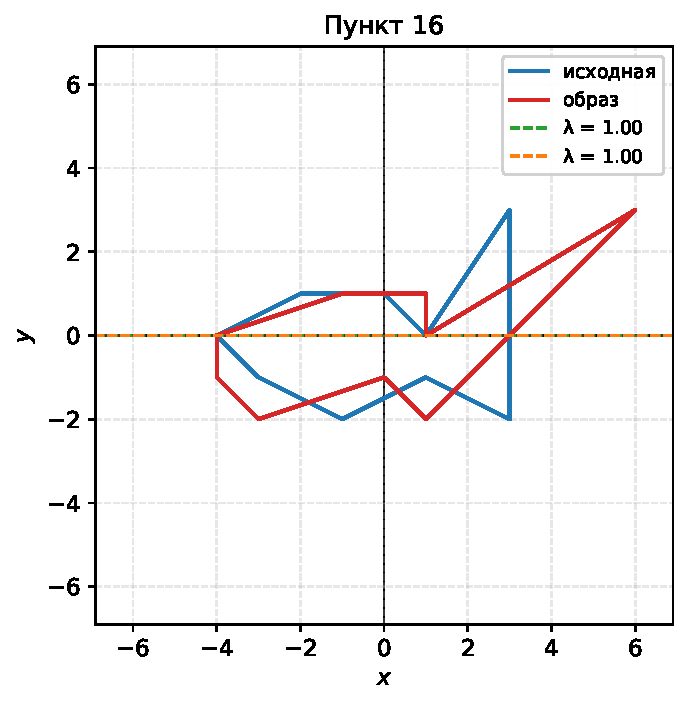
\includegraphics[width=0.55\textwidth]{../figures/p16A.pdf}
\caption{Пункт 16: отображение \(A\)}
\label{fig:p16A}
\end{figure}

\begin{figure}[H]
\centering
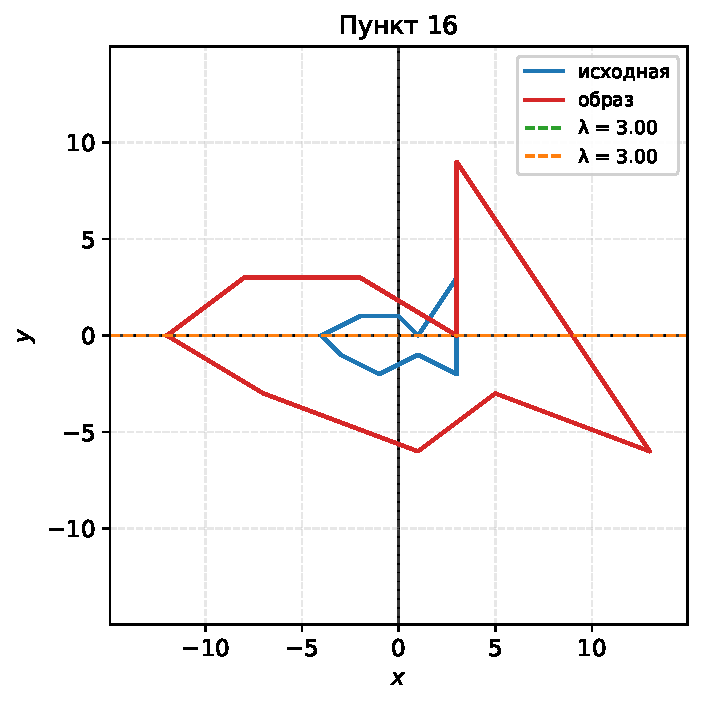
\includegraphics[width=0.55\textwidth]{../figures/p16B.pdf}
\caption{Пункт 16: отображение \(B\)}
\label{fig:p16B}
\end{figure}

\begin{figure}[H]
\centering
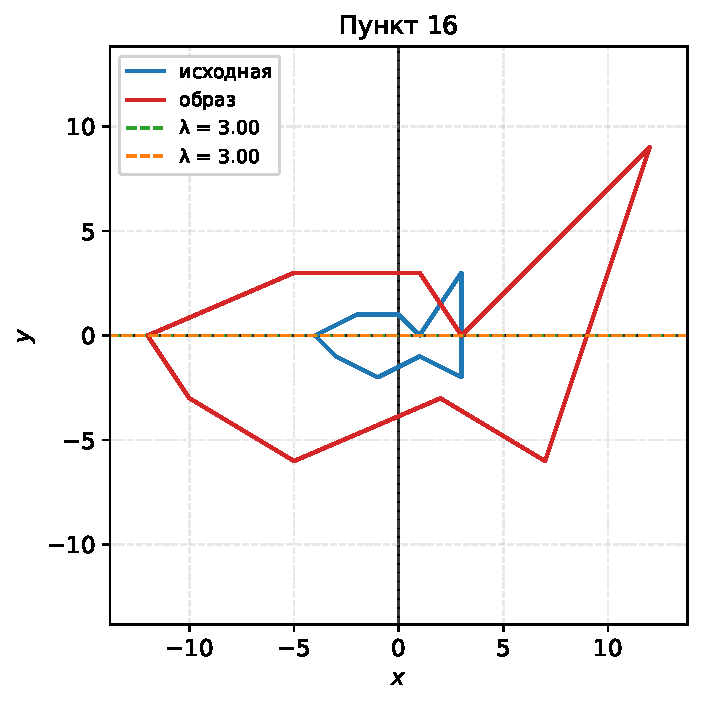
\includegraphics[width=0.55\textwidth]{../figures/p16AB.pdf}
\caption{Пункт 16: отображение \(AB\)}
\label{fig:p16AB}
\end{figure}

\begin{figure}[H]
\centering
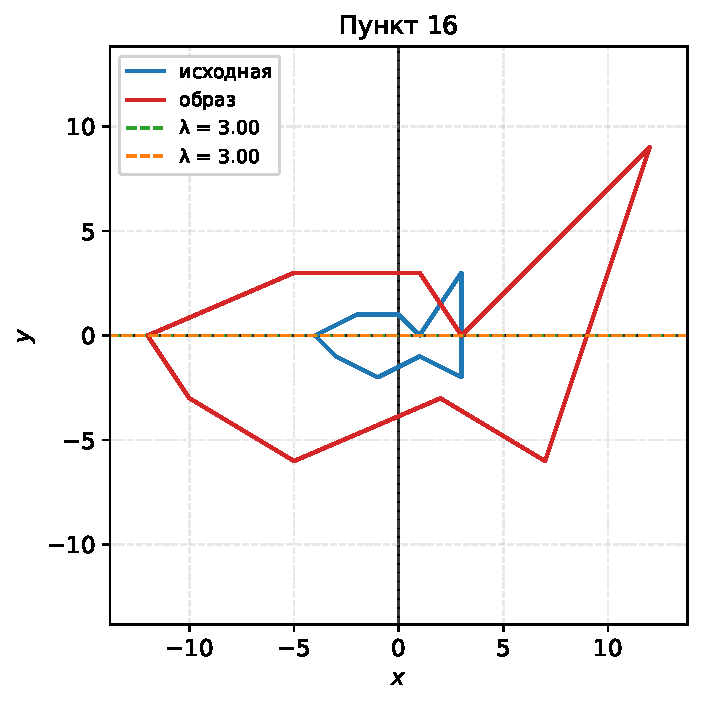
\includegraphics[width=0.55\textwidth]{../figures/p16BA.pdf}
\caption{Пункт 16: отображение \(BA\)}
\label{fig:p16BA}
\end{figure}

Так как \(AB=BA\), картинки \(AB\) и \(BA\) совпадут --- это визуально
демонстрирует коммутирование.

\textbf{Вывод.}\\
\(A_{16}\) и \(B_{16}\) максимально непохожи по диагонали, сдвигу и
определителю, но коммутируют: \begin{center}\adjustbox{max width=\linewidth}{$\displaystyle A_{16}B_{16}=B_{16}A_{16}.$}\end{center}

\begin{center}\rule{0.5\linewidth}{0.5pt}\end{center}

\hypertarget{ux441ux438ux43cux43cux435ux442ux440ux438ux447ux43dux43eux441ux442ux44c-ux438ux43dux432ux43eux43bux44eux442ux438ux432ux43dux43eux441ux442ux44c-ux43eux440ux442ux43eux433ux43eux43dux430ux43bux44cux43dux43eux441ux442ux44c}{%
\section{Симметричность, инволютивность,
ортогональность}\label{ux441ux438ux43cux43cux435ux442ux440ux438ux447ux43dux43eux441ux442ux44c-ux438ux43dux432ux43eux43bux44eux442ux438ux432ux43dux43eux441ux442ux44c-ux43eux440ux442ux43eux433ux43eux43dux430ux43bux44cux43dux43eux441ux442ux44c}}

Таблица 1 --- Свойства выбранных матриц (проверены в коде: \(M^T=M\),
\(M^2=I\), \(M^TM=I\))

\small\begin{longtable}{@{}p{1.3cm}p{5.0cm}p{2.8cm}p{2.8cm}p{2.8cm}@{}}
\toprule
Пункт & Отображение & Симметрична & Инволютивна &
Ортогональна\tabularnewline
\midrule
\endhead
1 & отражение относительно \(y=3x\) & да & да & да\tabularnewline
2 & ортогональная проекция на \(y=-2x\) & да & нет & нет\tabularnewline
3 & поворот на \(40^\circ\) & нет & нет & да\tabularnewline
4 & центральная симметрия & да & да & да\tabularnewline
5 & отражение, затем поворот & да & да & да\tabularnewline
6 & \(y=0\to y=3x\), \(x=0\to y=-2x\) & нет & нет & нет\tabularnewline
7 & \(y=3x\to y=0\), \(y=-2x\to x=0\) & нет & нет & нет\tabularnewline
8 & обмен прямых \(y=3x\) и \(y=-2x\) & нет & да & нет\tabularnewline
9 & круг \(\to\) круг площади 4 & нет & нет & нет\tabularnewline
10 & круг \(\to\) некруг площади 14 & нет & нет & нет\tabularnewline
11 & перпендикулярные собственные векторы & да & нет &
нет\tabularnewline
12 & жорданова клетка & нет & нет & нет\tabularnewline
13 & поворот на \(90^\circ\) & нет & нет & да\tabularnewline
14 & \(3I\) & да & нет & нет\tabularnewline
15 & \(A_{15},B_{15}\) & нет & нет & нет\tabularnewline
16 & \(A_{16},B_{16}\) & нет & нет & нет\tabularnewline
\bottomrule
\end{longtable}\normalsize

\textbf{Обязательно ли свойство следует из условия.}

\emph{Обязательно симметричны:} пункты 1, 2, 4, 11, 14. Отражение и
ортогональная проекция имеют ортогональные собственные векторы с
вещественными собственными числами, \(M=Q\Lambda Q^T\); в пункте 11
перпендикулярность собственных векторов --- само условие; \(-I\) и
\(\lambda I\) диагональны. Пункт 5 тоже получается симметричным, так как
это снова отражение.

\emph{Обязательно инволютивны:} пункты 1, 4, 5 --- отражения и
центральная симметрия: применённые дважды, они возвращают каждую точку
на место. В пункте 8 инволютивность --- свойство выбранной матрицы, а не
условия: обмен прямых может сопровождаться растяжением.

\emph{Обязательно ортогональны:} пункты 1, 3, 4, 5 --- отражения и
повороты сохраняют длины. В пункте 13 выбранный поворот ортогонален, но
условию «нет вещественных собственных векторов» удовлетворяют и
неортогональные матрицы (например, \(A_9\)). В пункте 9 при \(c=4\)
матрица \(A_9=2R_{30^\circ}\) не ортогональна, так как коэффициент
растяжения \(2\ne1\).


\unnumsection{Заключение}
В работе построены матрицы $2\times2$ для 16 геометрических преобразований плоскости. Почти все они
выводились одним приёмом: матрица однозначно задаётся тем, куда она переводит два неколлинеарных
вектора, поэтому удобно брать векторы, поведение которых известно из условия (вектор на прямой и
перпендикулярный ей), и находить $M = QP^{-1}$.

Определитель показал, как преобразование меняет площадь ($|\det M|$) и ориентацию (знак): у отражений
он равен $-1$, у поворотов и центральной симметрии $+1$, у проекции $0$ — плоскость схлопывается в прямую.
Собственные векторы оказались направлениями, которые матрица не сворачивает со своей прямой; у поворотов
их нет, собственные числа комплексные. Пункты 15 и 16 показали, что порядок применения преобразований
в общем случае важен: $AB \ne BA$.

\newpage
\unnumsection{Приложение А. Код}
\lstinputlisting[style=py,caption={Общий модуль \texttt{common.py}}]{../code/common.py}
\lstinputlisting[style=py,caption={Блок A: пункты 1--5}]{../code/block_a.py}
\lstinputlisting[style=py,caption={Блок B: пункты 6--8, 11, 12, 14}]{../code/block_b.py}
\lstinputlisting[style=py,caption={Блок C: пункты 9, 10, 13, 15, 16}]{../code/block_c.py}
\end{document}
